\documentclass[letterpaper,11pt]{article}

% --- PAQUETES DE IDIOMA
\usepackage[spanish,mexico]{babel}
\addto\captionsspanish{\renewcommand{\contentsname}{Indice}}
\usepackage[utf8]{inputenc}
\usepackage{pmboxdraw}
\usepackage{csquotes}
\usepackage{iftex}

\usepackage{pdfpages}

% --- PAQUETES MATEMÁTICOS --
\usepackage{amsmath}
\usepackage{cancel}
\usepackage{mathrsfs}

% --- PAQUETES GRÁFICOS Y DE DISEÑO ---
\usepackage{graphicx}
\usepackage{float}
\usepackage{placeins}
\usepackage{needspace}
\usepackage{subcaption}
\usepackage[table]{xcolor}
\usepackage{makecell}
\usepackage{array}
\usepackage{tikz}
\usetikzlibrary{shapes.geometric, shapes.multipart, positioning, arrows.meta, calc, shadows, decorations.pathreplacing,babel}

% --- LISTAS ---
\usepackage{enumitem}

% --- PAQUETES DE CÓDIGO ---
\usepackage{listings}
% Configuración del estilo de listings
\definecolor{codebg}{rgb}{0.95,0.95,0.95}   
\definecolor{keyword}{rgb}{0.0,0.2,0.6}     
\definecolor{comment}{rgb}{0.25,0.5,0.35}   
\definecolor{string}{rgb}{0.6,0.0,0.0}      
\definecolor{number}{rgb}{0.5,0.0,0.5}      
\definecolor{codegray}{rgb}{0.5,0.5,0.5}
\definecolor{codepurple}{rgb}{0.58,0,0.82}
\definecolor{backcolour}{rgb}{0.95,0.95,0.95}
\definecolor{cmdblue}{RGB}{0, 114, 188}
\definecolor{cmdred}{RGB}{204, 0, 0}       
\definecolor{cmdgreen}{RGB}{13, 165, 13}   
\definecolor{cmdgray}{RGB}{128, 128, 128} 
\definecolor{bgcode}{RGB}{248, 248, 248} 
\definecolor{bgTerminal}{RGB}{30, 30, 30}
\definecolor{textTerminal}{RGB}{230, 230, 230}




\lstset{
  backgroundcolor=\color{backcolour},
  basicstyle=\ttfamily\small,
  keywordstyle=\color{blue}\bfseries,
  stringstyle=\color{codepurple},
  commentstyle=\color{codegray}\itshape,
  numbers=left,
  numberstyle=\tiny\color{codegray},
  frame=single,
  rulecolor=\color{black},
  breaklines=true,
  tabsize=4,
  showstringspaces=false,
  literate={á}{{\'a}}1
           {é}{{\'e}}1
           {í}{{\'i}}1
           {ó}{{\'o}}1
           {ú}{{\'u}}1
           {Á}{{\'A}}1
           {É}{{\'E}}1
           {Í}{{\'I}}1
           {Ó}{{\'O}}1
           {Ú}{{\'U}}1
           {ñ}{{\~n}}1
           {Ñ}{{\~N}}1
           {¿}{{\textquestiondown}}1
           {¡}{{\textexclamdown}}1
}

% Estilo para código en C
\lstdefinestyle{cstyle}{
  language=C,
  backgroundcolor=\color{backcolour},
  basicstyle=\ttfamily\small,
  keywordstyle=\color{blue}\bfseries,
    keywordstyle=[2]\color{yellow!70!orange}\bfseries,
    morekeywords=[2]{MPI_Init,MPI_Comm_size,MPI_Comm_rank,MPI_Send,MPI_Recv,MPI_Scatter,MPI_Gather,MPI_Bcast,MPI_Reduce,MPI_Finalize},
    emph={printf},
    emphstyle=\color{blue}\bfseries,
  stringstyle=\color{codepurple},
  commentstyle=\color{codegray}\itshape,
  numbers=left,
  numberstyle=\tiny\color{codegray},
  frame=single,
  rulecolor=\color{black},
  breaklines=true,
  tabsize=4,
  showstringspaces=false
}

\lstdefinestyle{salidaLinpeas}{
    basicstyle=\ttfamily\scriptsize\color{textTerminal},
    backgroundcolor=\color{bgTerminal},
    breaklines=true,
    breakatwhitespace=true,
    frame=single,
    rulecolor=\color{black!50},
    numbers=none,
    showstringspaces=false,
    tabsize=4,
    xleftmargin=0.5cm,
    xrightmargin=0.5cm,
    extendedchars=false,
    literate={═}{{\textSFxliii}}1
             {║}{{\textSFxxiv}}1
             {╔}{{\textSFxxxix}}1
             {╗}{{\textSFxxv}}1
             {╚}{{\textSFxxxviii}}1
             {╝}{{\textSFxxvi}}1
             {╣}{{\textSFxxiii}}1
}  
\lstdefinestyle{consolaSeguridad}{
    language=bash,
    basicstyle=\ttfamily\footnotesize,
    backgroundcolor=\color{bgcode},
    % Herramientas y comandos de la práctica
    morekeywords={subfinder, make, scp, httpx, hydra, ssh, id, nuclei, dig, whois, grep, awk, sort, cut, sed, tr, nano, wc, head, echo, sudo, nmap, wget, curl, ip,
                  whoami, file, cat, cp, chown, chmod, sha256sum, apt-get, john, unshadow, su, pwnkit, uname, uniq, ps, route, ifconfig, find, tar, ping, nc, ls, bash},
    alsoletter={-},
    keywordstyle=\color{cmdblue}\bfseries,
    % Palabras reservadas de ciclos Bash
    emph={for, in, do, done, while, read, if, then, fi},
    emphstyle=\color{cmdred}\bfseries,
    stringstyle=\color{cmdgreen},
    commentstyle=\color{cmdgray}\itshape,
    showstringspaces=false,
    breaklines=true,
    breakatwhitespace=false,
    frame=single,
    rulecolor=\color{black!30},
    numbers=none,
    literate={-}{{\textcolor{black}{-}}}1
             {ñ}{{\~n}}1
             {Ñ}{{\~N}}1
}

% Definición del lenguaje Python para listings
\lstdefinelanguage[LAB]{Python}{
    morekeywords={False, None, True, and, as, assert, async, await, break,
                                class, continue, def, del, elif, else, except, finally,
                                for, from, global, if, import, in, is, lambda, nonlocal,
                                not, or, pass, raise, return, try, while, with, yield,
                                machine, Pin, PWM, ADC, Timer, sleep_ms, sleep_us},
    morecomment=[l]{\#},
    morestring=[b]",
    morestring=[b]',
    sensitive=true
}

% Definición del lenguaje Makefile para listings
\lstdefinelanguage{Makefile}{
    morekeywords={all, setup, clean, conversion-mod.so, pwnkit},
    morecomment=[l]{\#},
    morestring=[b]',
    morestring=[b]",
    sensitive=true
}

% Estilo para salidas de consola/terminal
\lstdefinestyle{output}{
  backgroundcolor=\color{black!5},
  basicstyle=\ttfamily\footnotesize,
  numbers=none,
  frame=single,
  rulecolor=\color{black!30},
  breaklines=true,
  tabsize=4,
  showstringspaces=false,
  xleftmargin=0.5cm,
  xrightmargin=0.5cm
}

% --- ESTILOS PARA DIAGRAMAS DE FLUJO (TIKZ) ---
\tikzset{
  startstop/.style={rectangle, rounded corners, minimum width=3cm, minimum height=1cm,text centered, draw=black, fill=red!30},
  process/.style={rectangle, minimum width=3cm, minimum height=1cm, text centered, draw=black, fill=orange!30},
  decision/.style={diamond, aspect=2, minimum width=3cm, minimum height=1cm, text centered, draw=black, fill=green!30},
  io/.style={trapezium, trapezium left angle=70, trapezium right angle=110, minimum width=3cm, minimum height=1cm, text centered, draw=black, fill=blue!30},
  arrow/.style={thick,->,>=stealth}
}


\definecolor{azulresultado}{HTML}{0072C6}
\definecolor{rojoacarreo}{HTML}{FF0000}

% --- RUTAS DE IMÁGENES ---
\graphicspath{{img/}{portada_img/}}

\definecolor{armblue}{RGB}{0, 113, 188}

% --- ÍNDICE CON PUNTOS ---
\usepackage{tocloft}
\renewcommand{\cftsecleader}{\cftdotfill{\cftdotsep}}

% --- CONFIGURACIÓN DE PÁGINA (GEOMETRÍA) ---
\usepackage[
    left=25mm, 
    right=25mm,
    top=35mm,
    bottom=30mm,
    headheight=77pt, 
    papersize={21.59cm,27.94cm}
]{geometry}

% --- FORMATO DE TEXTO ---
\usepackage{setspace}
\onehalfspacing
\usepackage{parskip} 
\usepackage{lipsum}  

% --- VARIABLES GLOBALES ---
\newcommand{\materia}{}

% --- ENCABEZADOS Y PIES DE PÁGINA ---
\usepackage{fancyhdr}
\pagestyle{fancy}
\fancyhf{} 
\fancyhead[L]{
\includegraphics[height=1.5cm]{portada_img/der.png}}
\fancyhead[R]{
\includegraphics[height=1.5cm]{portada_img/izq.png}}
\fancyfoot[C]{\thepage} 

\renewcommand{\headrulewidth}{0.4pt} 
\renewcommand{\footrulewidth}{0pt}  

% --- BIBLIOGRAFÍA ---
\usepackage[backend=biber, style=apa, sortcites, url=true]{biblatex}
\addbibresource{referencias.bib}

% --- HIPERVÍNCULOS ---
\usepackage{hyperref}
\hypersetup{
    colorlinks=true,
    linkcolor=blue,
    citecolor=blue,
    filecolor=magenta,
    urlcolor=cyan
}


\fancypagestyle{estiloindice}{
  \fancyhf{} 
  \fancyhead[L]{
\includegraphics[height=1.5cm]{portada_img/der.png}}
  \fancyhead[R]{
\includegraphics[height=1.5cm]{portada_img/izq.png}}
  \renewcommand{\headrulewidth}{0.4pt} 
  \renewcommand{\footrulewidth}{0pt}
}


% --- CADENAS DE HASHES: CONSERVAR CARACTERES Y PERMITIR SALTOS ---
\lstdefinestyle{hashCredencial}{
  style=output,
  basicstyle=\ttfamily\footnotesize,
  columns=fullflexible,
  keepspaces=true,
  breaklines=true,
  breakatwhitespace=false,
  xleftmargin=0pt,
  xrightmargin=0pt,
  postbreak=\mbox{\textcolor{codegray}{$\hookrightarrow$}\space}
}

\begin{document}
\setlength{\emergencystretch}{1em}
\hypersetup{pageanchor=false}
\thispagestyle{empty} % Sin encabezado ni pie en la portada

% --- ENCABEZADO DE PORTADA (TABLA DE 3 COLUMNAS) ---
\begin{center}
    % La tabla usa 'm' para centrar verticalmente las imagenes y el texto
    \begin{tabular}{m{0.15\textwidth} m{0.60\textwidth} m{0.15\textwidth}}
        % Logo Izquierdo (UNAM)
        
\includegraphics[width=2cm]{portada_img/der.png} & 
        
        % Titulo Central
        \centering\Huge\textbf{Universidad Nacional Autonoma de Mexico} &
        
        % Logo Derecho (Facultad)
        \raggedleft
\includegraphics[width=2cm]{portada_img/izq.png}
    \end{tabular}
\end{center}

\vspace{0.3cm}

% --- INFORMACION DEL REPORTE ---
\begin{center}
    {\LARGE \textbf{Facultad de Ingenieria}}\\[1cm]

    {\LARGE \textbf{Alumno:}}\\[0.3cm]
    {\Large Lara Hernandez Angel Husiel - 320060829} \\[1cm]


    {\LARGE \textbf{Seguridad informatica basica}} \\[1cm]

	{\LARGE Semestre: 2027-1} \\[1cm]
    
    {\LARGE \textbf{Practica 6}}\\[0.5cm]

    {\LARGE {Discovery}}\\[1cm]


    {\Large \textbf{Fecha de Entrega:}}\\[0.2cm]
    {\Large 31 de Octubre del 2026 }
\end{center}
\newpage
{\hypersetup{linkcolor=black}\tableofcontents}
\thispagestyle{estiloindice}
\newpage
\thispagestyle{fancy}
\setcounter{page}{1}
\hypersetup{pageanchor=true}
\singlespacing
\section{Desarrollo}

\subsection{Identificacion de la direccion IP y revision de conectividad}

Ahora bien, primero revisamos la
direccion IP de nuestra maquina EvilBox, esto por que necesitamos
identificar el segmento de red en el que se encuentra webserver.


\begin{lstlisting}[style=consolaSeguridad]
ip a
\end{lstlisting}

Donde en este caso, la interfaz \texttt{ens33} tiene la direccion
\texttt{192.168.177.128/24}, por lo que la red que vamos a revisar
es \texttt{192.168.177.0/24}. Despues de esto, ponemos el
siguiente comando:

\begin{lstlisting}[style=consolaSeguridad]
sudo nmap 192.168.177.0/24
\end{lstlisting}

\begin{figure}[H]
    \centering
    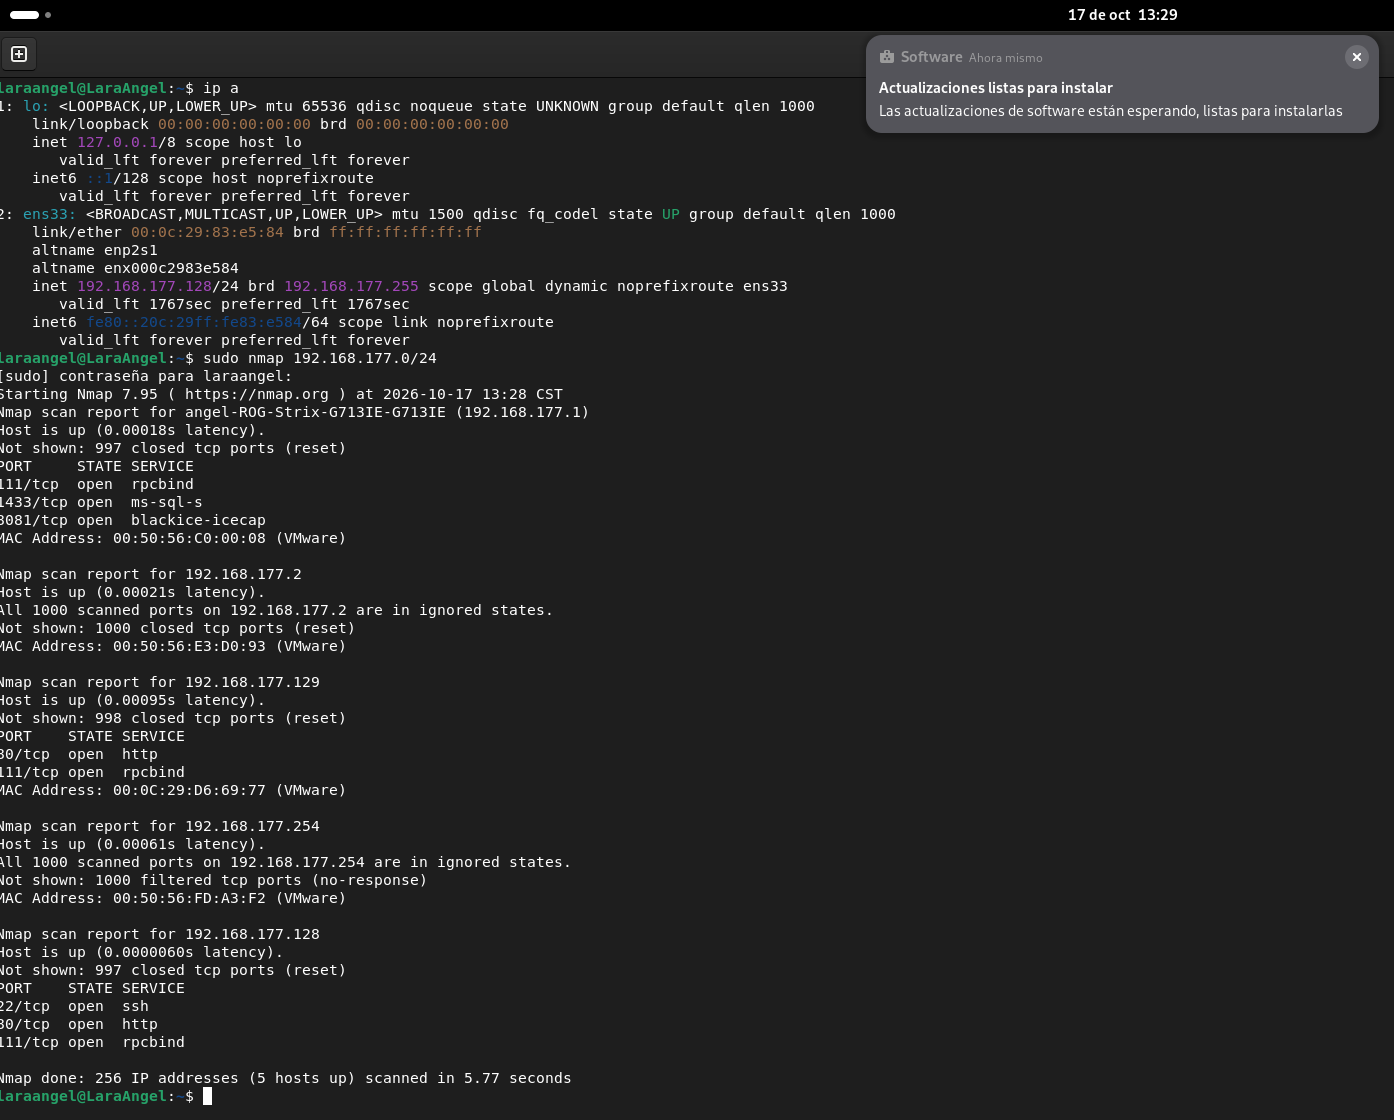
\includegraphics[width=0.9\textwidth]{img/image2.png}
    \caption{Revision de la direccion IP y escaneo del segmento de red.}
\end{figure}

Lo que hace nmap es revisar los equipos del segmento y los puertos
TCP mas comunes. Donde \texttt{sudo} permite ejecutarlo con
permisos de administracion y \texttt{/24} indica que se esta
trabajando con la mascara \texttt{255.255.255.0}. En este caso se
hizo el escaneo normal, por lo que ademas de encontrar equipos
activos tambien se obtuvo informacion de sus puertos.

La salida nos arroja cinco equipos activos. Donde el servidor al
que nos vamos a conectar es \texttt{192.168.177.129}, siendo esta
la misma direccion de webserver que se utilizo en las practicas
anteriores. El equipo codeserver se va a buscar despues desde la
otra red a la que tiene acceso webserver.

\subsection{Conexion por SSH y cambio al usuario root}

Para poder conectarnos a webserver, utilizamos el usuario y la
contraseña que se obtuvieron en la practica 3. Recordando que el
usuario es webadmin, la contraseña es toronto y el puerto SSH es
el 13337, el comando completo es el siguiente:

\begin{lstlisting}[style=consolaSeguridad]
ssh webadmin@192.168.177.129 -p 13337
\end{lstlisting}

Donde \texttt{ssh} permite abrir la sesion remota y la bandera
\texttt{-p} indica el puerto por el que se realiza la conexion.
Despues en la consola se pone la contraseña, siendo
\texttt{toronto}. En el primer intento se rechazo la contraseña y
al ingresarla de nuevo se logro establecer la conexion.

\begin{figure}[H]
    \centering
    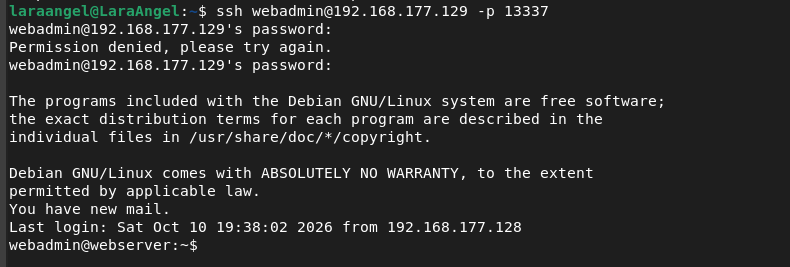
\includegraphics[width=\textwidth]{img/image3.png}
    \caption{Conexion por SSH al servidor con el usuario webadmin.}
\end{figure}

Ahora bien, para continuar es necesario cambiar al usuario root.
Para esto ya tenemos la contraseña que se obtuvo con John en la
practica 5, siendo \texttt{Maverick}, con la M mayuscula. El
comando que utilizamos es el siguiente:

\begin{lstlisting}[style=consolaSeguridad]
su root
\end{lstlisting}

Despues de escribir la contraseña, comprobamos el usuario con el
comando whoami:

\begin{lstlisting}[style=consolaSeguridad]
whoami
\end{lstlisting}

\begin{lstlisting}[style=output]
root
\end{lstlisting}

\begin{figure}[H]
    \centering
    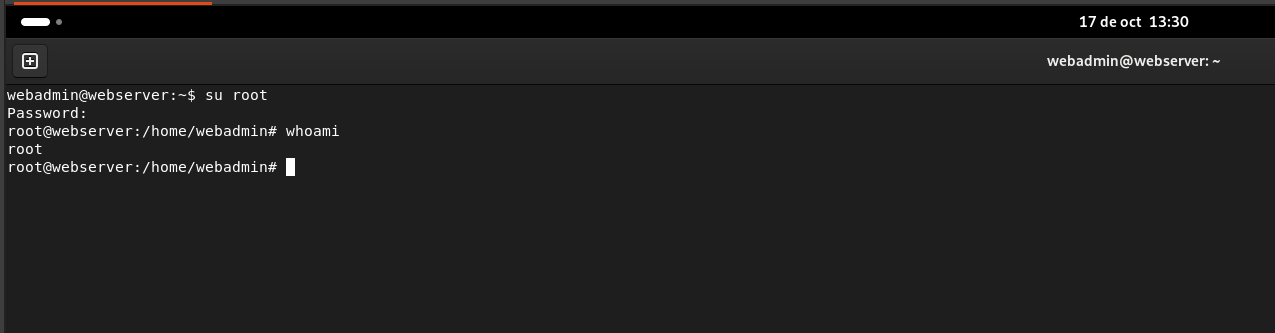
\includegraphics[width=\textwidth,trim=0bp 105bp 0bp 0bp,clip]{img/image4.png}
    \caption{Cambio al usuario root y comprobacion con whoami.}
\end{figure}

Donde en este caso, whoami nos arroja root, por lo que ya tenemos
los permisos necesarios para revisar la informacion del equipo.

\Needspace{12\baselineskip}
\subsection{Informacion del sistema}

Para poder identificar las caracteristicas de webserver, primero
revisamos la version de compilacion del kernel. Para esto,
utilizamos el comando siguiente:

\Needspace{6\baselineskip}
\begin{lstlisting}[style=consolaSeguridad]
uname -v
\end{lstlisting}

\begin{lstlisting}[style=output]
#1 SMP Debian 3.16.56-1+deb8u1 (2018-05-08)
\end{lstlisting}

Lo que hace \texttt{uname} es mostrar informacion del sistema,
donde la bandera \texttt{-v} nos da la version de compilacion del
kernel. En este caso nos devuelve una compilacion de Debian
identificada como \texttt{3.16.56-1+deb8u1}.

Despues de esto, revisamos los archivos que contienen la
informacion de la distribucion. El comando es el siguiente:

\begin{lstlisting}[style=consolaSeguridad]
cat /etc/*release | uniq
\end{lstlisting}

Donde \texttt{cat} muestra el contenido de los archivos de
\texttt{/etc} que terminan en release, el simbolo \texttt{*}
permite completar esa parte del nombre y la tuberia \texttt{|}
pasa la salida a \texttt{uniq}, el cual quita las lineas repetidas
que se encuentran una junto a otra.

\begin{lstlisting}[style=output]
PRETTY_NAME="Debian GNU/Linux 8 (jessie)"
NAME="Debian GNU/Linux"
VERSION_ID="8"
VERSION="8 (jessie)"
ID=debian
\end{lstlisting}

\begin{figure}[H]
    \centering
    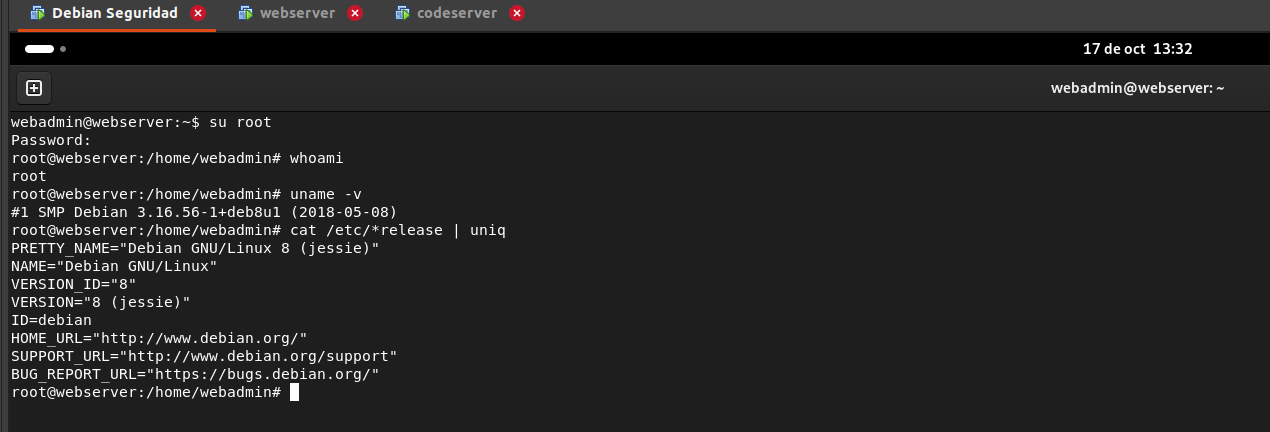
\includegraphics[width=\textwidth]{img/image5.png}
    \caption{Version de compilacion del kernel e informacion de Debian.}
\end{figure}

Con esto podemos ver que el equipo utiliza Debian GNU/Linux 8, con
el nombre jessie. Donde \texttt{PRETTY\_NAME} es el nombre
completo de la distribucion, mientras que \texttt{VERSION\_ID}
indica el numero de version.

\Needspace{12\baselineskip}
\subsection{Revision de los procesos en ejecucion}

Ahora bien, para conocer los programas que se estan ejecutando en
webserver.

\Needspace{6\baselineskip}
\begin{lstlisting}[style=consolaSeguridad]
ps aux awf
\end{lstlisting}

Lo que hace ps es mostrar los procesos activos en ese momento. Las
opciones \texttt{a} y \texttt{x} permiten incluir procesos de
otros usuarios y procesos que no tienen una terminal asociada;
\texttt{u} agrega informacion del usuario y los recursos,
\texttt{w} amplia la salida y \texttt{f} muestra la relacion entre
los procesos en forma de arbol.

\begin{figure}[H]
    \centering
    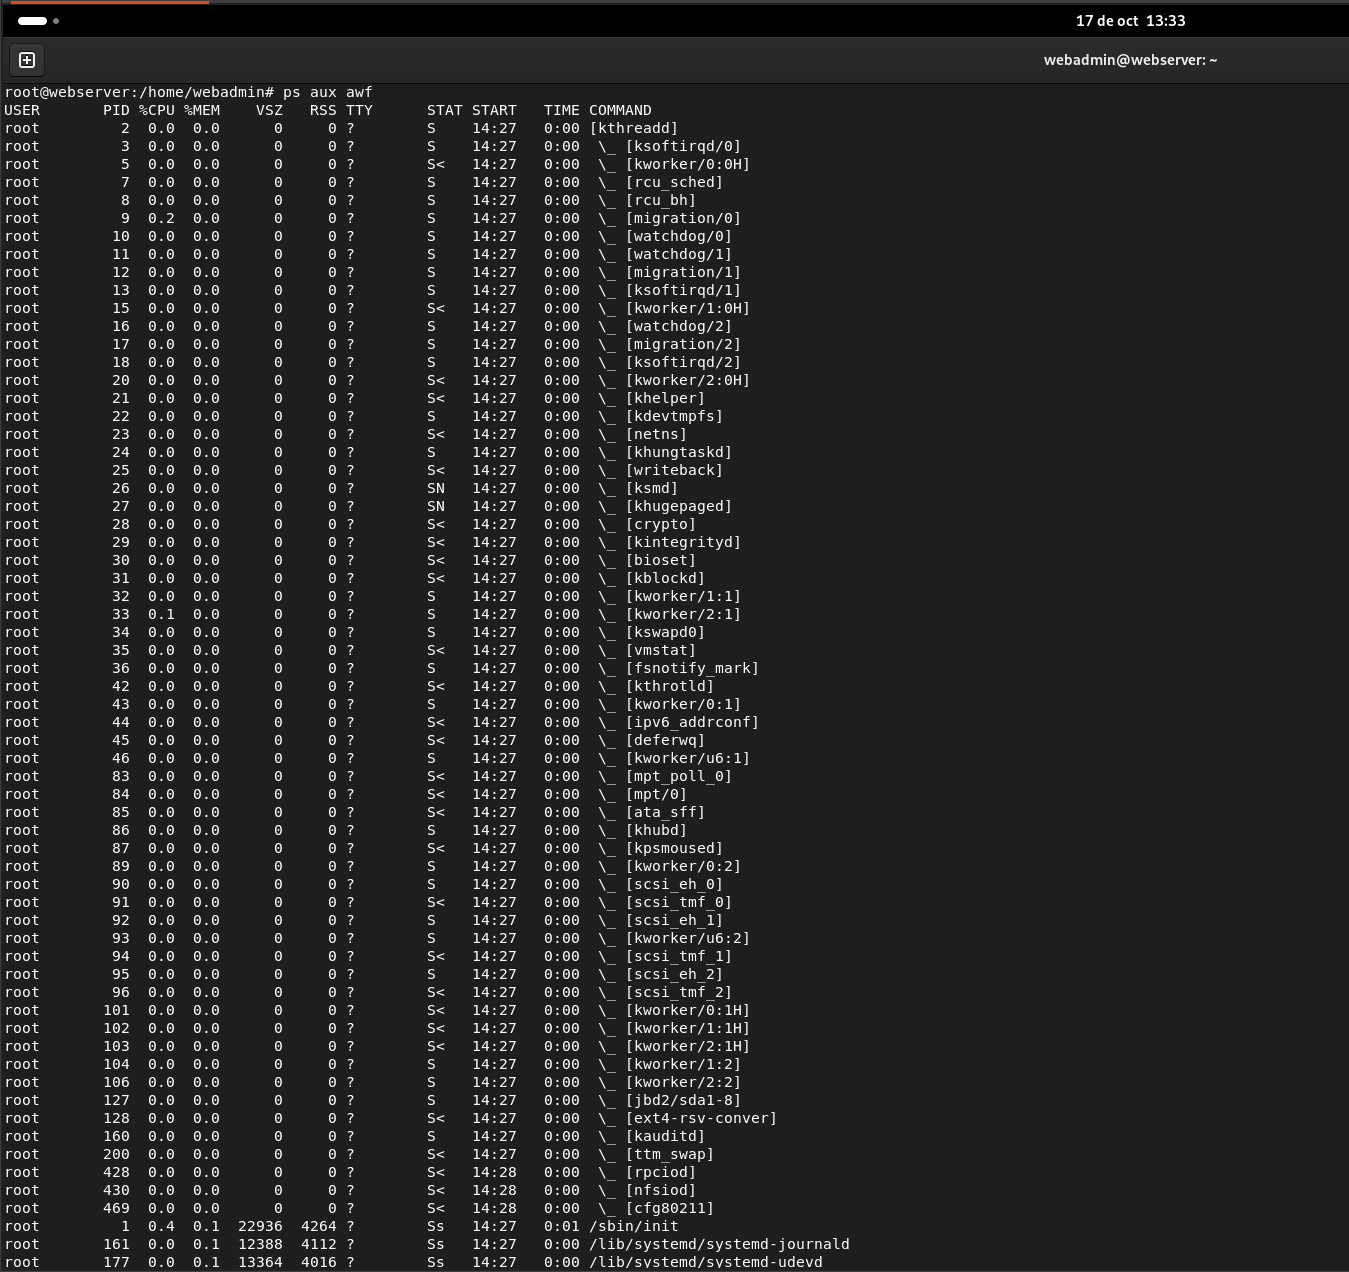
\includegraphics[width=\textwidth,trim=0bp 650bp 250bp 55bp,clip]{img/image6.png}
    \caption{Listado de procesos y columnas de informacion del sistema.}
\end{figure}



Donde en este caso, los dos servicios que nos interesan son SSH y
Apache. Para SSH se identifica el comando \texttt{/usr/sbin/sshd
-D}, mientras que para Apache se encuentra
\texttt{/usr/sbin/apache2 -k start}.

\begin{figure}[H]
    \centering
    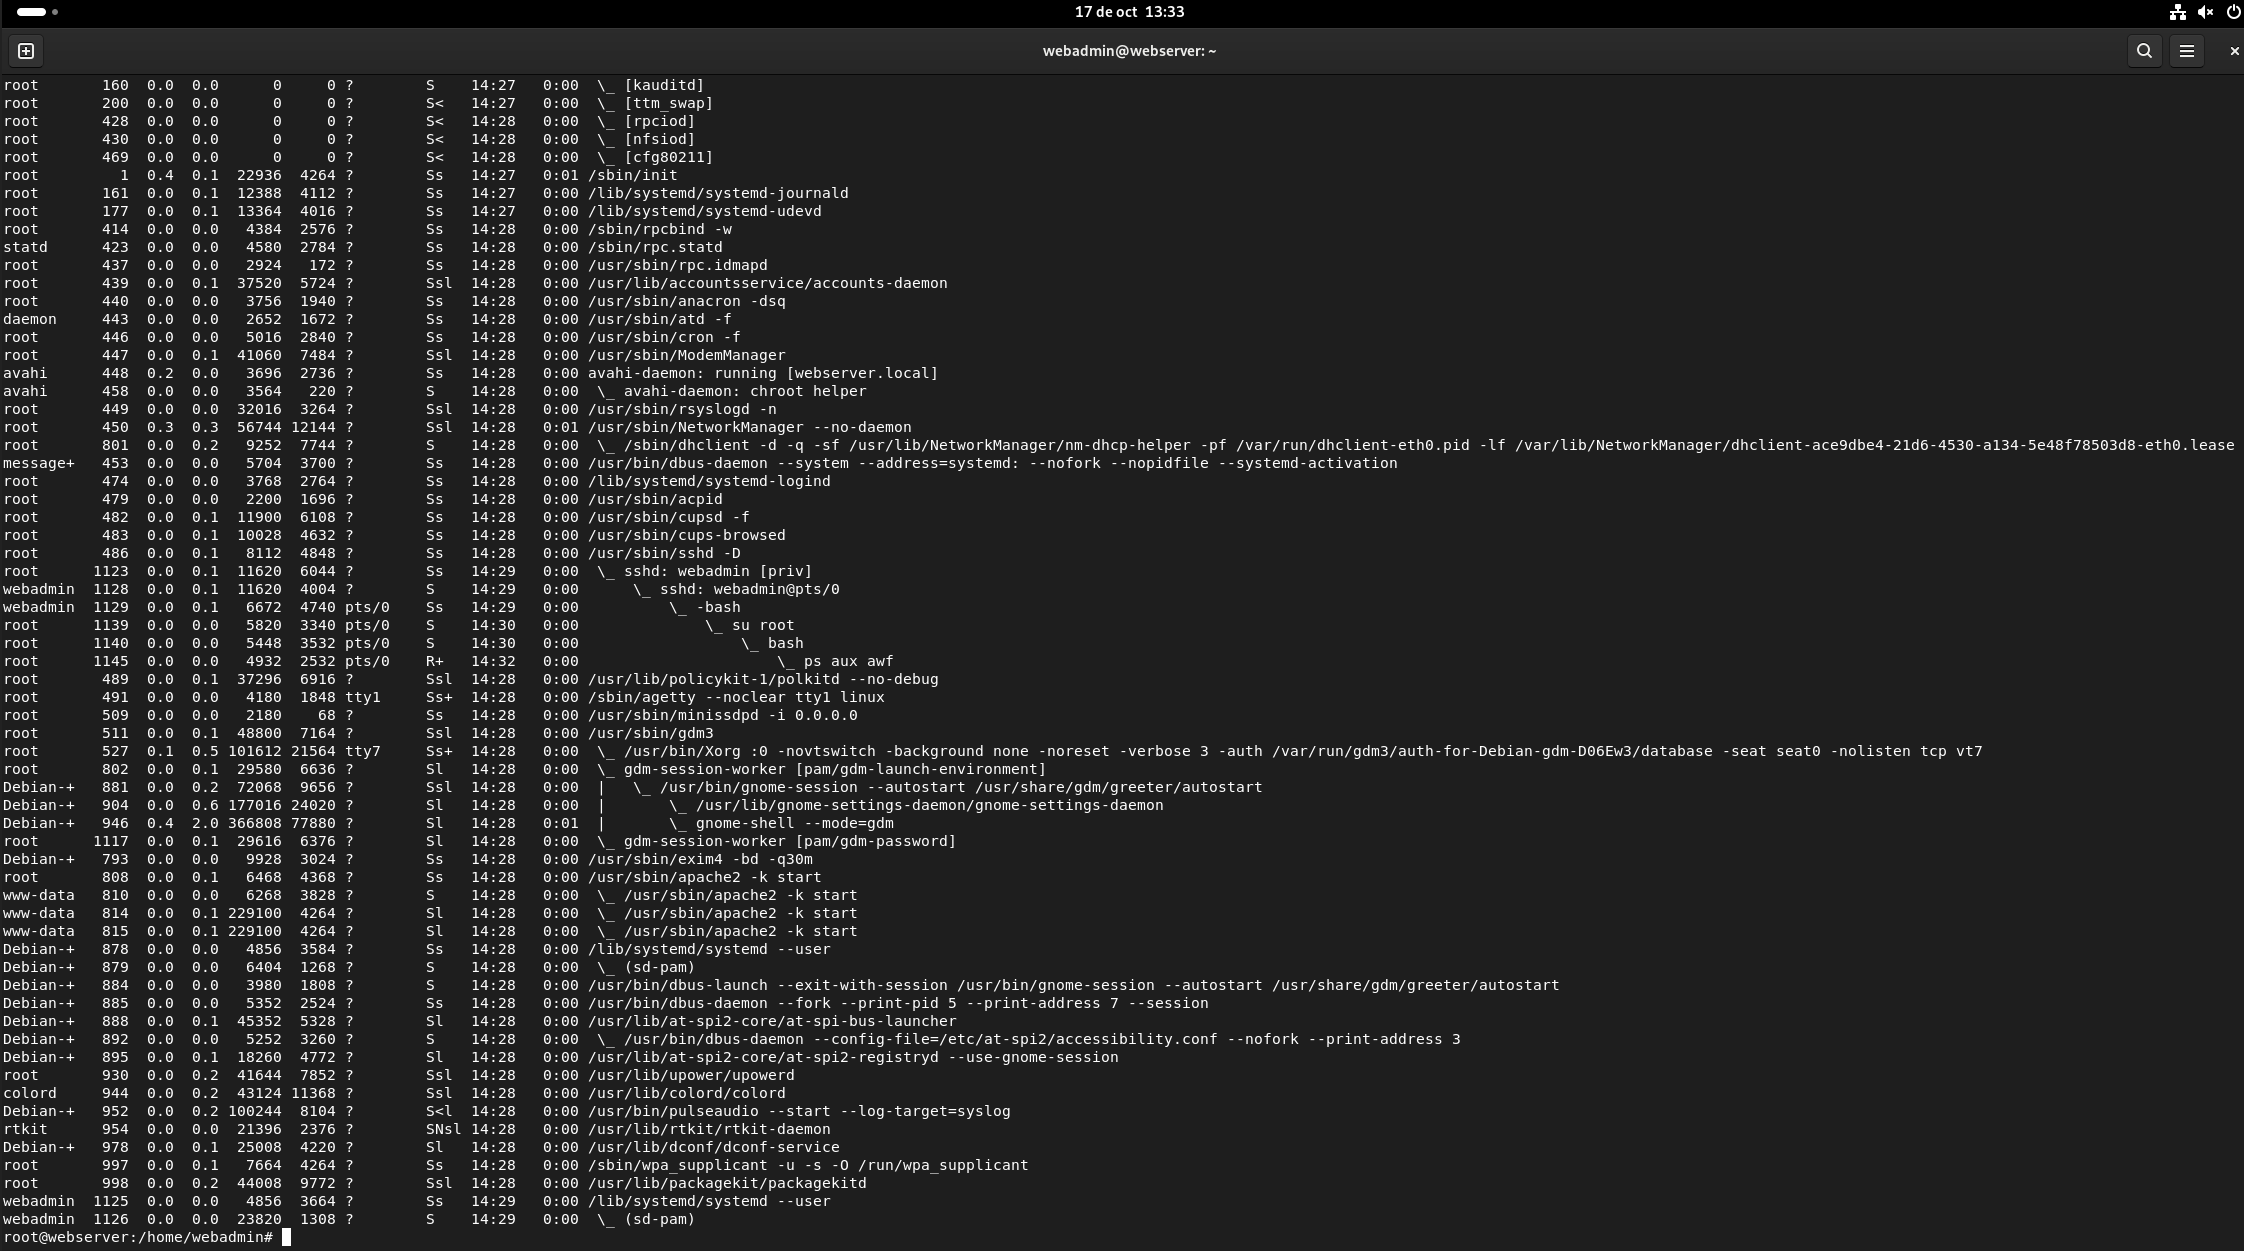
\includegraphics[width=\textwidth,trim=0bp 300bp 850bp 480bp,clip]{img/image7.png}
    \caption{Procesos de los servicios SSH y Apache en webserver.}
\end{figure}

El proceso principal de SSH tiene el PID 486 y se ejecuta como
root. Para Apache, el proceso principal tiene el PID 808 y sus
procesos hijos se ejecutan como www-data. Ademas de que, por medio
del arbol tambien se puede relacionar la conexion SSH con la
terminal que se esta utilizando.

\subsection{Revision de la configuracion de red}

\subsubsection{Tabla de rutas}

Para poder identificar a que redes tiene acceso el servidor,
primero revisamos la tabla de rutas con el siguiente comando:

\begin{lstlisting}[style=consolaSeguridad]
route -n
\end{lstlisting}

Donde \texttt{route} muestra las rutas del equipo y \texttt{-n}
mantiene las direcciones en forma numerica, sin intentar resolver
nombres. El resultado es el siguiente:

\begin{lstlisting}[style=output]
Destination     Gateway     Genmask         Flags  Iface
0.0.0.0         10.0.0.1    0.0.0.0         UG     eth1
10.0.0.0        0.0.0.0    255.255.255.0   U      eth1
192.168.177.0   0.0.0.0    255.255.255.0   U      eth0
\end{lstlisting}

Con esto podemos ver que eth0 esta conectada a la red
\texttt{192.168.177.0/24}, mientras que eth1 esta conectada a
\texttt{10.0.0.0/24}. Ademas de que, la ruta por defecto utiliza la puerta de
enlace \texttt{10.0.0.1}. La bandera U indica que la ruta esta
activa y G que utiliza una puerta de enlace.

\subsubsection{Archivo hosts}

Despues de esto, revisamos las asociaciones locales entre
direcciones y nombres, esto por medio del siguiente comando:

\begin{lstlisting}[style=consolaSeguridad]
cat /etc/hosts
\end{lstlisting}

El archivo contiene las entradas \texttt{127.0.0.1 localhost} y
\texttt{127.0.1.1 webserver}, ademas de las entradas de IPv6. Esto
permite identificar el nombre local del servidor, pero no es un
listado de todos los equipos que estan conectados a la red.

\subsubsection{Interfaces del servidor}

Para revisar las direcciones asignadas a cada interfaz, utilizamos
el siguiente comando:

\begin{lstlisting}[style=consolaSeguridad]
ifconfig -a
\end{lstlisting}

Donde la bandera \texttt{-a} permite mostrar todas las interfaces,
incluyendo las que no estan activas. En este caso se encuentran
tres interfaces, siendo eth0, eth1 y lo.

\begin{figure}[H]
    \centering
    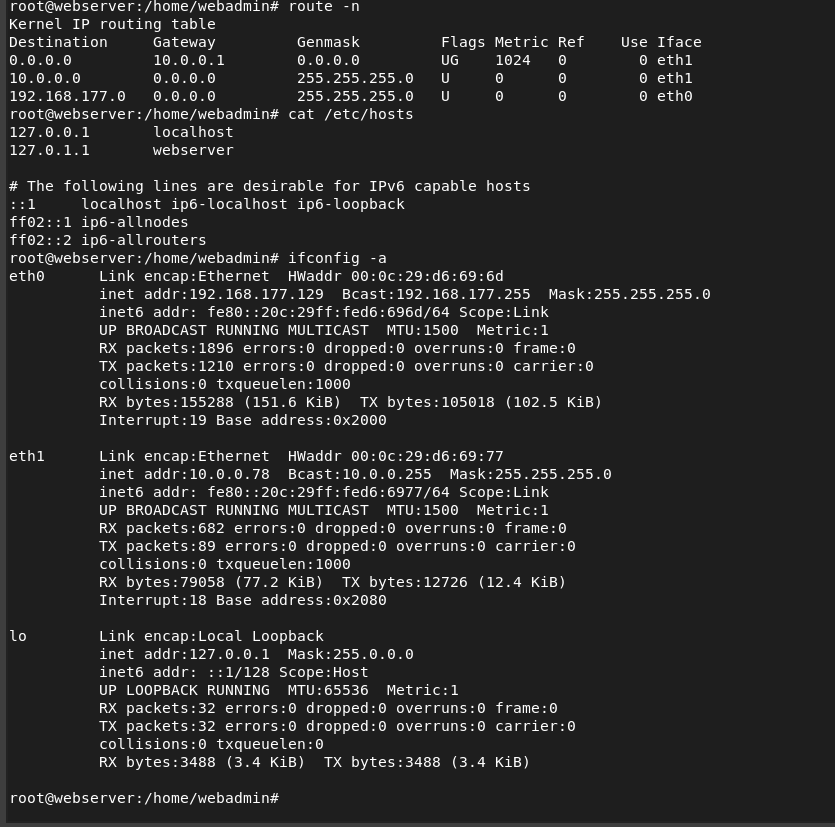
\includegraphics[width=0.9\textwidth]{img/image8.png}
    \caption{Tabla de rutas, archivo hosts e interfaces de red de webserver.}
\end{figure}

\begin{center}
\begin{tabular}{|l|l|l|}
\hline
\textbf{Interfaz} & \textbf{Direccion IPv4} & \textbf{Mascara} \\ \hline
eth0 & 192.168.177.129 & 255.255.255.0 \\ \hline
eth1 & 10.0.0.78 & 255.255.255.0 \\ \hline
lo & 127.0.0.1 & 255.0.0.0 \\ \hline
\end{tabular}
\end{center}

Donde eth0 es la interfaz por la que nos conectamos desde EvilBox
y eth1 es la que nos permite revisar la red interna
\texttt{10.0.0.0/24}.

\subsection{Busqueda de archivos y directorios}

\subsubsection{Busqueda por extensiones y nombres de archivo}

Ahora bien, para encontrar archivos que puedan tener informacion
importante, utilizamos find. Lo que hace este comando es recorrer
los directorios a partir de la ruta que se indique y buscar los
nombres que coincidan con una condicion. Primero ponemos lo
siguiente:

\begin{lstlisting}[style=consolaSeguridad]
find /home/webadmin -name "*.pdf"
\end{lstlisting}

Donde \texttt{/home/webadmin} es el directorio desde el que se
busca y \texttt{-name} compara el nombre del archivo. En este caso
no se encontro ningun PDF con ese patron dentro de ese directorio.

\begin{figure}[H]
    \centering
    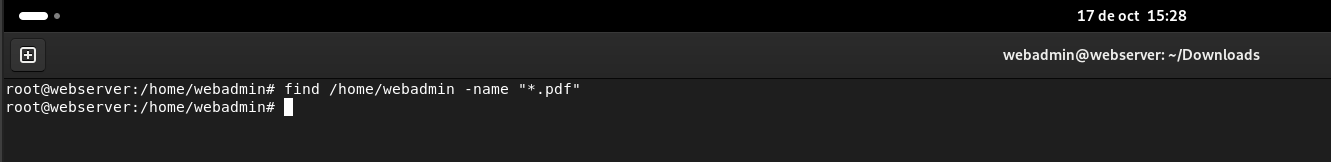
\includegraphics[width=\textwidth]{img/parte9Desarrollo/image1.png}
    \caption{Busqueda de archivos PDF dentro del directorio de webadmin.}
\end{figure}

Despues de esto ampliamos la busqueda a los archivos de Python,
utilizando el comando siguiente:

\begin{lstlisting}[style=consolaSeguridad]
find / -name "*.py" 2>/dev/null
\end{lstlisting}

Para esto, \texttt{/} indica que la busqueda empieza desde la raiz
del sistema y \texttt{*.py} permite encontrar nombres que terminen
con esa extension. Las comillas evitan que la terminal complete el
patron antes de pasarlo a find. Por otro lado,
\texttt{2>/dev/null} descarta los mensajes de error, conservando
los resultados de la busqueda.

\begin{figure}[H]
    \centering
    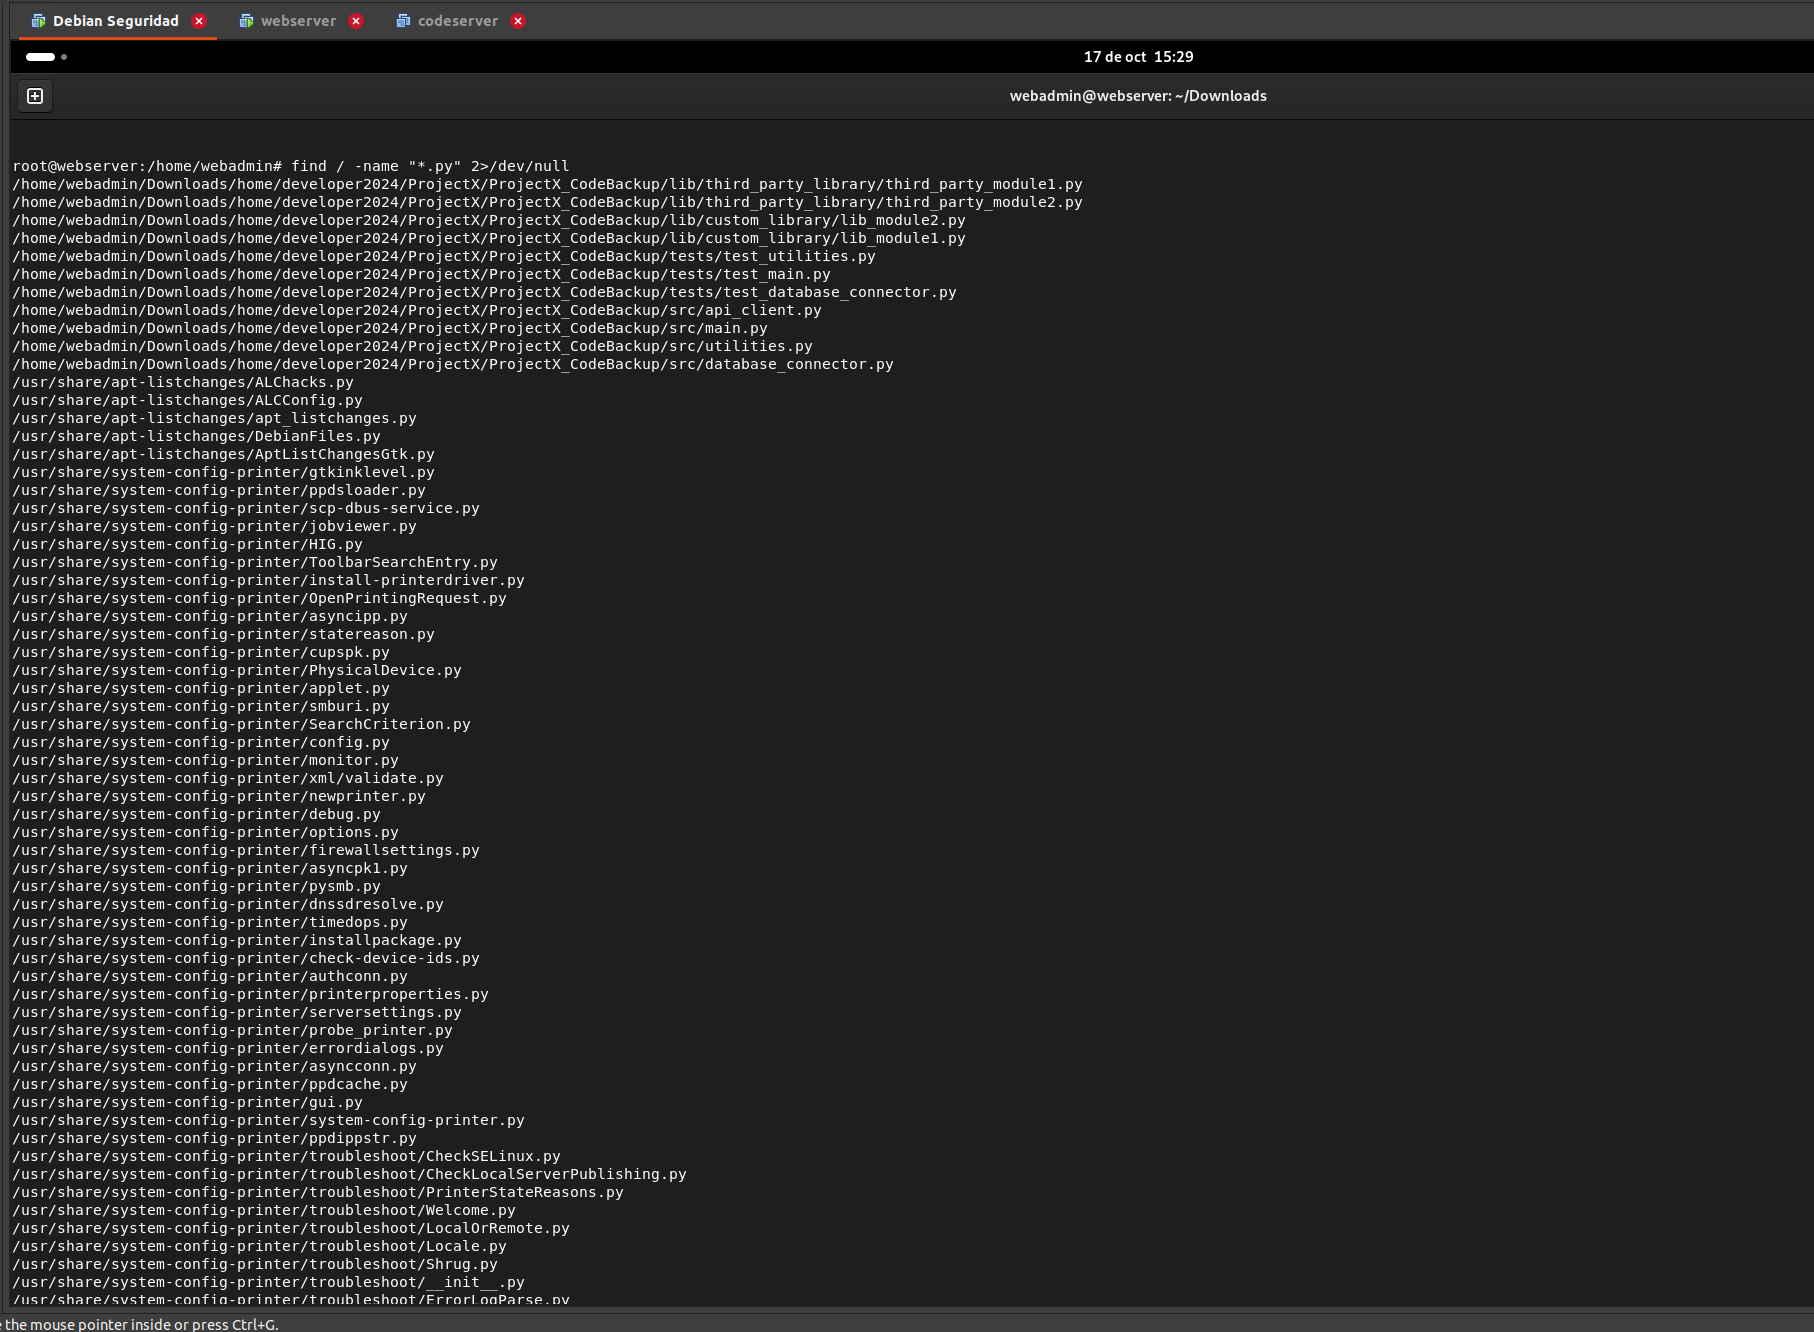
\includegraphics[width=0.95\textwidth]{img/parte9Desarrollo/image2.png}
    \caption{Busqueda de archivos de Python en el sistema.}
\end{figure}

La busqueda devuelve archivos del sistema y varios archivos de un
proyecto llamado ProjectX. Donde en este caso, dentro de Downloads
se encuentra el directorio \texttt{ProjectX\_CodeBackup}, con
archivos como main.py, api\_client.py y database\_connector.py,
por lo que esta ruta nos sirve para continuar revisando el
respaldo del proyecto.

De igual forma, se buscaron documentos de Word y nombres de
archivo relacionados con contraseñas o respaldos. Los comandos son
los siguientes:

\begin{lstlisting}[style=consolaSeguridad]
find / -name "*.docx" 2>/dev/null
find /root -name "contraseñas.txt" 2>/dev/null
find / -name "passwords.xlsx" 2>/dev/null
find / -name "respaldo.zip" 2>/dev/null
\end{lstlisting}

Donde en este caso, estas cuatro busquedas no devolvieron
coincidencias. Para buscar dentro del directorio del usuario root
se utilizo \texttt{/root}, que es la ruta que tiene este usuario
en el servidor.

\begin{figure}[H]
    \centering
    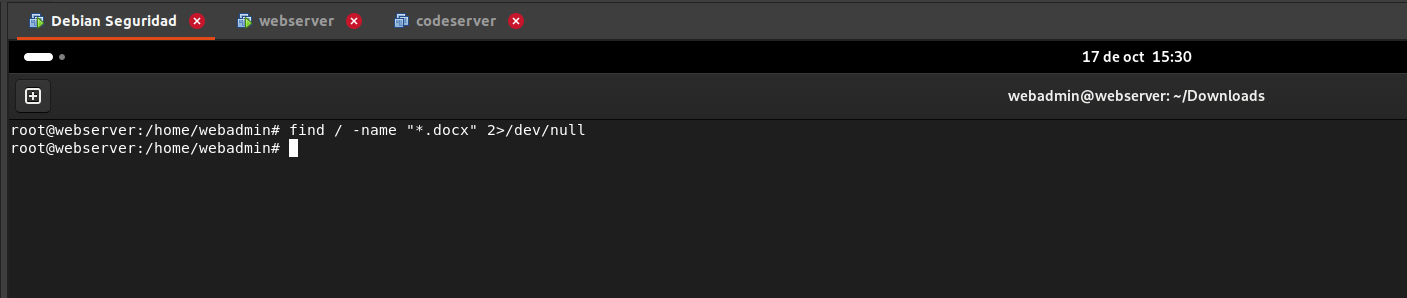
\includegraphics[width=\textwidth]{img/parte9Desarrollo/image3.png}
    \caption{Busqueda de archivos con extension docx.}
\end{figure}

\begin{figure}[H]
    \centering
    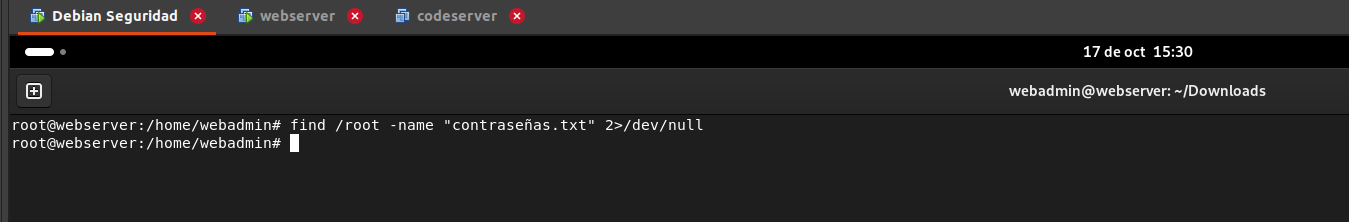
\includegraphics[width=\textwidth]{img/parte9Desarrollo/image4.png}
    \caption{Busqueda del archivo contraseñas.txt en el directorio de root.}
\end{figure}

\begin{figure}[H]
    \centering
    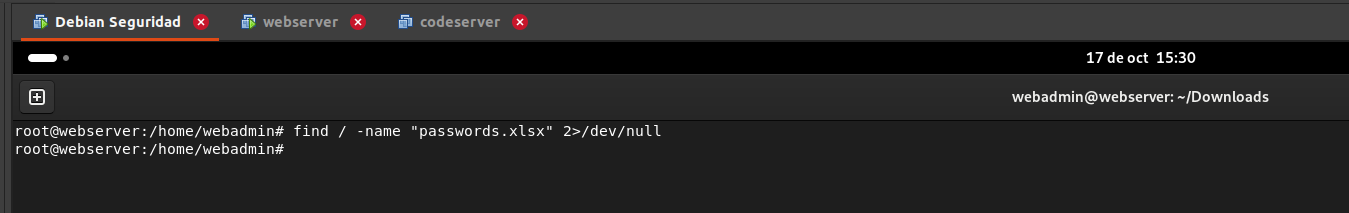
\includegraphics[width=\textwidth]{img/parte9Desarrollo/image5.png}
    \caption{Busqueda del archivo passwords.xlsx.}
\end{figure}

\begin{figure}[H]
    \centering
    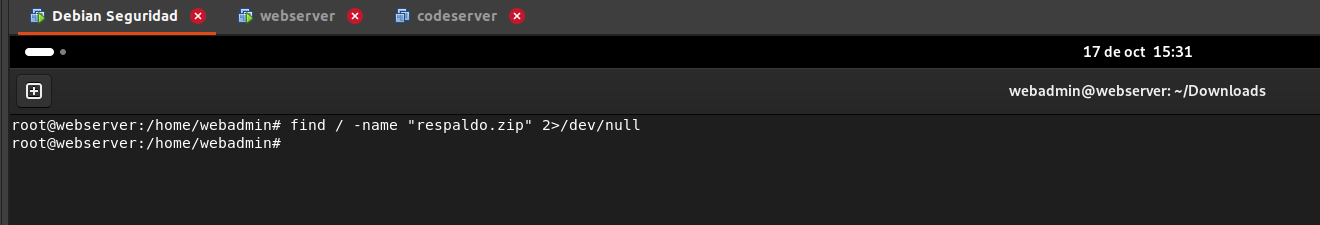
\includegraphics[width=\textwidth]{img/parte9Desarrollo/image6.png}
    \caption{Busqueda del archivo respaldo.zip.}
\end{figure}

Ademas de las busquedas por nombre exacto, se ampliaron los
patrones para buscar cualquier archivo con extension xlsx y zip:

\begin{lstlisting}[style=consolaSeguridad]
find / -name "*.xlsx" 2>/dev/null
find / -name "*.zip" 2>/dev/null
\end{lstlisting}

Para xlsx no se obtuvieron coincidencias. En el caso de zip
aparecieron archivos de librerias y paquetes del sistema, pero
esos nombres por si solos no comprueban que contengan contraseñas.

\subsubsection{Busqueda de respaldos comprimidos}

Para continuar con los archivos comprimidos, revisamos los que
tienen la extension tar.gz. Para esto, el comando es el siguiente:

\begin{lstlisting}[style=consolaSeguridad]
find / -name "*.tar.gz" 2>/dev/null
\end{lstlisting}

\begin{figure}[H]
    \centering
    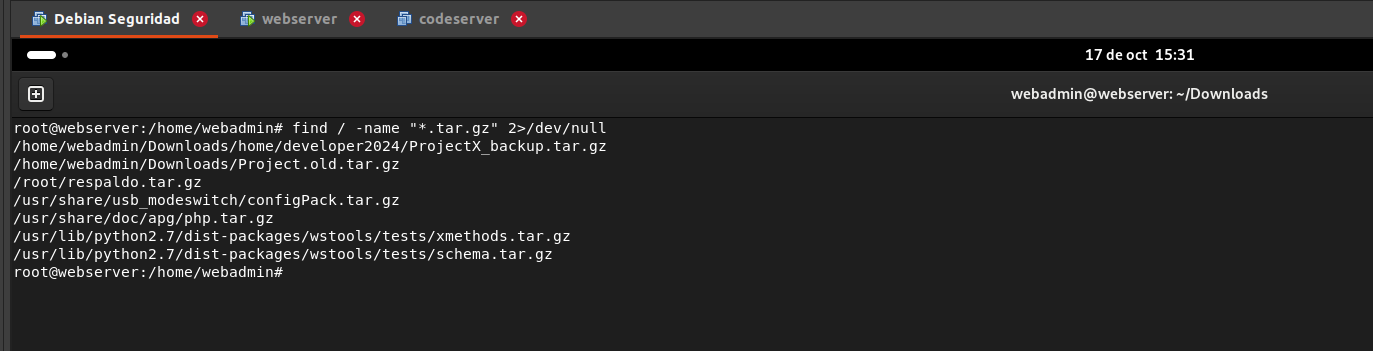
\includegraphics[width=\textwidth]{img/parte9Desarrollo/image7.png}
    \caption{Busqueda de respaldos y otros archivos con extension tar.gz.}
\end{figure}

Donde en este caso, los archivos que nos interesan son los
siguientes:

\begin{lstlisting}[style=output]
/home/webadmin/Downloads/home/developer2024/ProjectX_backup.tar.gz
/home/webadmin/Downloads/Project.old.tar.gz
/root/respaldo.tar.gz
\end{lstlisting}

No obstante, tambien se reviso si habia algun respaldo antiguo
dentro de var, utilizando el siguiente comando:

\begin{lstlisting}[style=consolaSeguridad]
find /var -name "*old.tar.gz" 2>/dev/null
\end{lstlisting}

\begin{figure}[H]
    \centering
    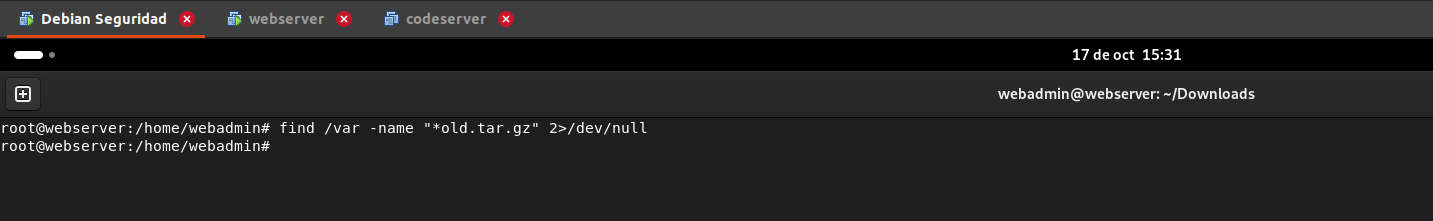
\includegraphics[width=\textwidth]{img/parte9Desarrollo/image8.png}
    \caption{Busqueda de respaldos antiguos dentro de var.}
\end{figure}

Esta busqueda no devolvio coincidencias dentro de var. Con esto,
continuamos con los respaldos que ya se habian encontrado en
Downloads y en el directorio de root.

\subsubsection{Busqueda de nombres relacionados con contraseñas}

Ahora bien, buscar solamente un nombre exacto puede dejar fuera
otros archivos. Para ampliar la busqueda utilizamos las siguientes
variaciones:

\begin{lstlisting}[style=consolaSeguridad]
find / -type f -iname "*pass*.txt" 2>/dev/null
find / -type f -iname "*cred*.txt" 2>/dev/null
find / -type f -iname "*contra*.txt" 2>/dev/null
find / -type f -iname "*claves*" 2>/dev/null
\end{lstlisting}

Donde \texttt{-type f} permite buscar archivos regulares y
\texttt{-iname} compara los nombres sin distinguir entre
mayusculas y minusculas. Los asteriscos permiten que la palabra
buscada se encuentre en cualquier parte del nombre.

\begin{figure}[H]
    \centering
    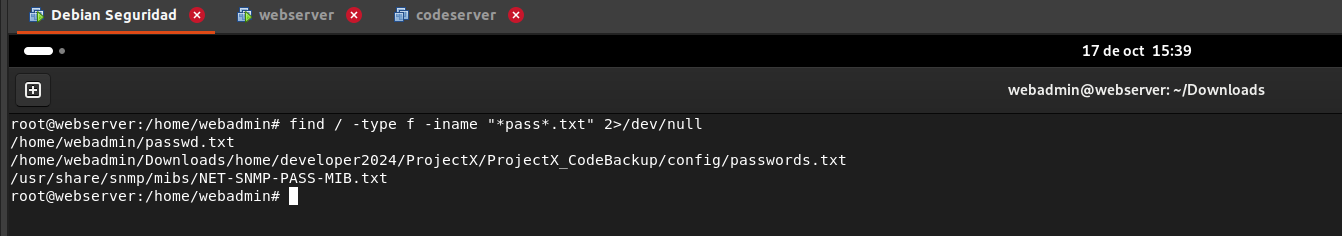
\includegraphics[width=\textwidth]{img/parte9Desarrollo/image9.png}
    \caption{Busqueda de archivos de texto con pass en el nombre.}
\end{figure}

Para el patron pass se encontraron tres rutas, incluyendo
passwd.txt, que ya se habia utilizado en la practica 5, y un
archivo llamado passwords.txt dentro del respaldo de ProjectX.
Este segundo archivo es el que vamos a revisar para comprobar si
tiene contraseñas en claro.

\begin{figure}[H]
    \centering
    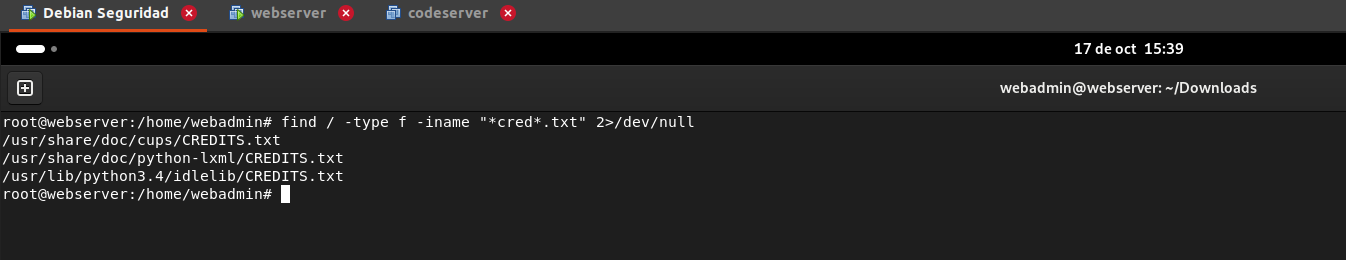
\includegraphics[width=\textwidth]{img/parte9Desarrollo/image10.png}
    \caption{Busqueda de archivos de texto con cred en el nombre.}
\end{figure}

\begin{figure}[H]
    \centering
    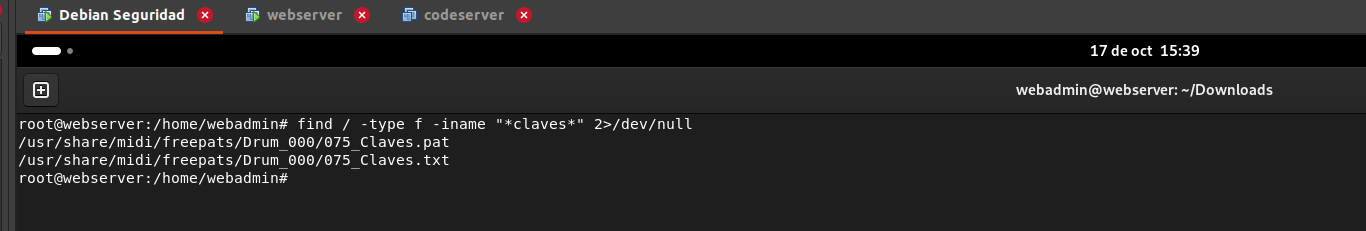
\includegraphics[width=\textwidth]{img/parte9Desarrollo/image11.png}
    \caption{Busqueda de archivos con claves en el nombre.}
\end{figure}

Por otro lado, cred devolvio archivos CREDITS.txt y claves
encontro archivos de un instrumento musical llamado Claves. Para
contra no se obtuvieron resultados. Con esto podemos ver que
encontrar una palabra en el nombre no significa que el archivo
contenga credenciales; es necesario revisar su contenido.

\subsubsection{Revision de los respaldos y del archivo passwords.txt}

Para ver el contenido de los respaldos sin extraerlos de nuevo,
utilizamos tar con las siguientes opciones:

\begin{lstlisting}[style=consolaSeguridad]
tar -ztvf /root/respaldo.tar.gz
tar -ztvf /home/webadmin/Downloads/Project.old.tar.gz
\end{lstlisting}

Donde \texttt{-z} permite leer la compresion gzip, \texttt{-t}
lista el contenido, \texttt{-v} agrega informacion de los archivos
y \texttt{-f} indica el archivo que se va a revisar. En
respaldo.tar.gz aparece flag2.txt, mientras que Project.old.tar.gz
contiene la estructura del proyecto, incluyendo el directorio
config y el archivo passwords.txt.

Despues de esto, para revisar el archivo que ya se encuentra
dentro de Downloads, se utiliza el comando siguiente:

\begin{lstlisting}[style=consolaSeguridad]
cat /home/webadmin/Downloads/home/developer2024/ProjectX/ProjectX_CodeBackup/config/passwords.txt
\end{lstlisting}

\begin{figure}[H]
    \centering
    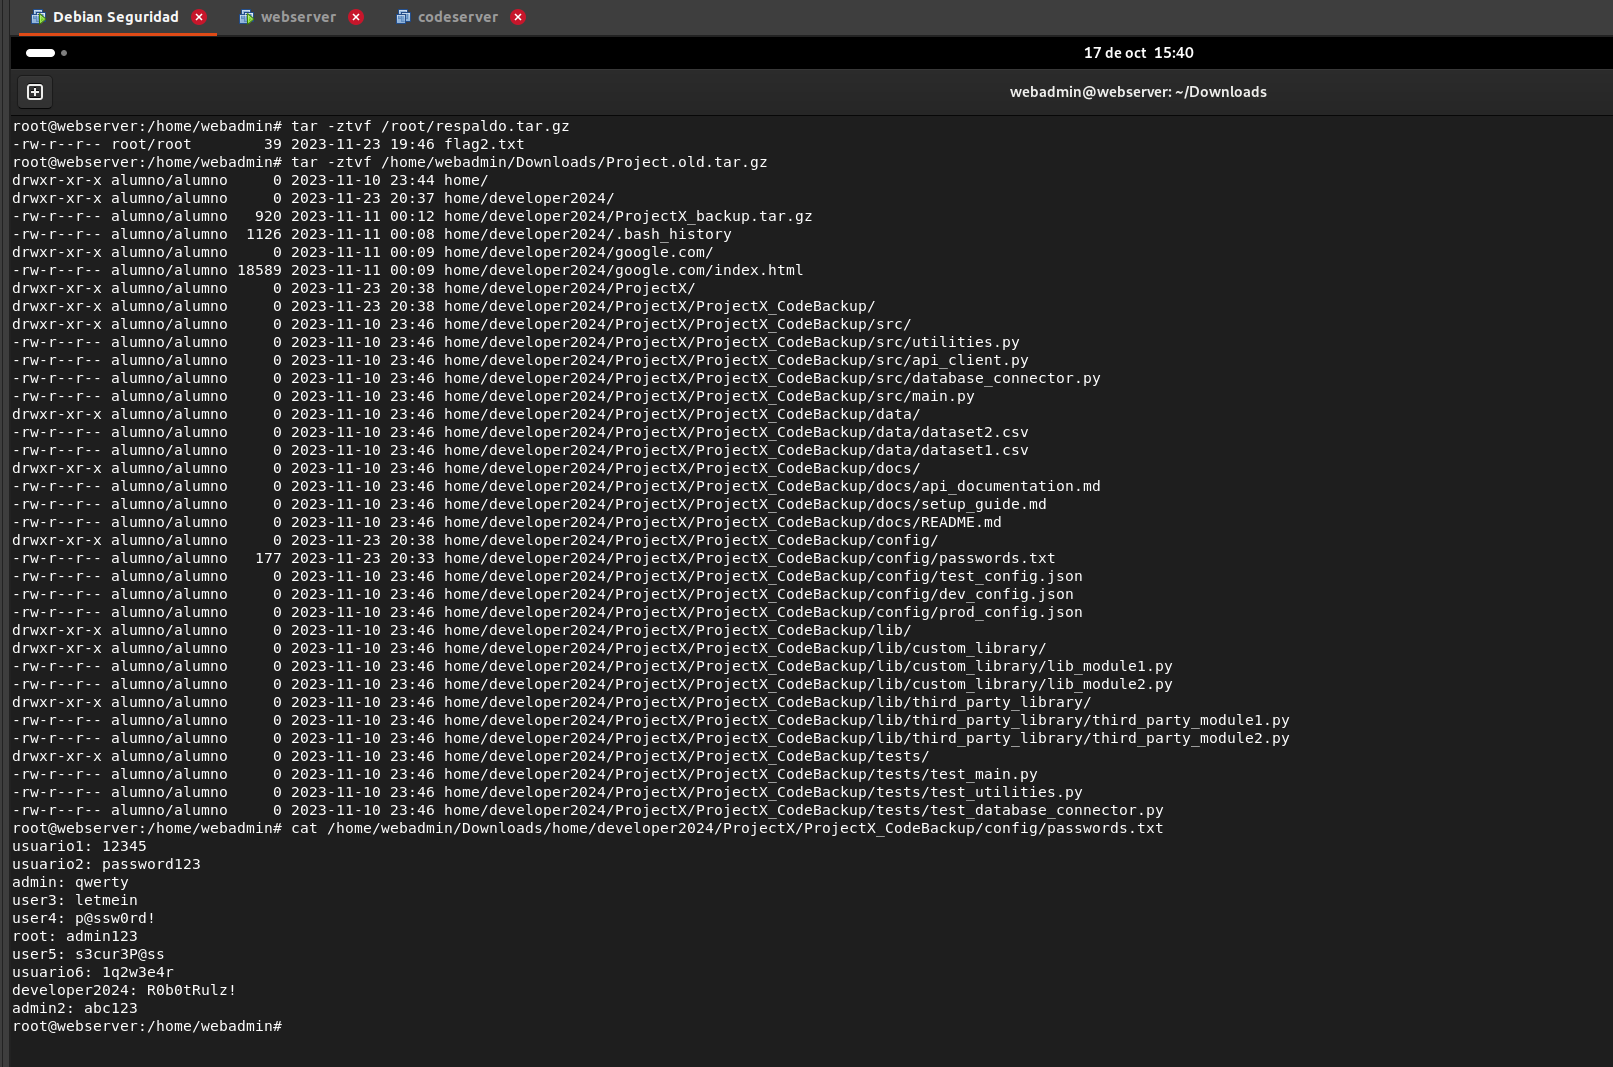
\includegraphics[width=\textwidth]{img/parte9Desarrollo/image12.png}
    \caption{Revision de los respaldos y lectura del archivo passwords.txt.}
\end{figure}

Donde en este caso, el archivo contiene diez pares de usuario y
contraseña escritos directamente en texto. El contenido es el
siguiente:

\begin{lstlisting}[style=output]
usuario1: 12345
usuario2: password123
admin: qwerty
user3: letmein
user4: p@ssw0rd!
root: admin123
user5: s3cur3P@ss
usuario6: 1q2w3e4r
developer2024: R0b0tRulz!
admin2: abc123
\end{lstlisting}

Con esto se comprueba que el archivo si contiene contraseñas en
claro, ya que se pueden leer sin realizar un proceso como el que
se utilizo con John. No obstante, la entrada root: admin123
pertenece al archivo del respaldo y no demuestra que esa sea la
contraseña actual del usuario root de webserver, donde la
contraseña que utilizamos fue Maverick.

\subsubsection{Busqueda de cadenas dentro de los archivos}

Por ultimo, ademas de buscar por nombre, tambien se reviso el
contenido de varios directorios. Para esto se utilizo grep con el
siguiente comando:

\begin{lstlisting}[style=consolaSeguridad]
grep -rnI --exclude="linpeas*" -iE "pass|contra|clave|user|admin" /root/ /home/webadmin/ /var/www/ /opt/ /etc/ 2>/dev/null
\end{lstlisting}

Donde \texttt{-r} hace la busqueda de forma recursiva, \texttt{-n}
agrega el numero de linea, \texttt{-I} omite archivos binarios,
\texttt{-i} no distingue entre mayusculas y minusculas y
\texttt{-E} permite utilizar la expresion con varias palabras
separadas por \texttt{|}. Ademas de que,
\texttt{--exclude="linpeas*"} deja fuera los archivos cuyo nombre
empieza con linpeas.

Esta busqueda devolvio coincidencias del archivo passwords.txt,
junto con comentarios, configuraciones y otros archivos del
sistema. Por lo que no todas las coincidencias corresponden a una
contraseña; para esta practica el archivo que se comprobo fue el
del respaldo de ProjectX.

\subsection{Construccion y transferencia del escaner de red}

Ahora bien, como webserver tiene la interfaz eth1 en otra red, lo
que vamos a hacer es revisar que otros equipos se encuentran
conectados a ese segmento. Para esto se preparo un archivo llamado
escaner.sh en EvilBox, utilizando el comando siguiente:

\begin{lstlisting}[style=consolaSeguridad]
nano escaner.sh
\end{lstlisting}

\Needspace{22\baselineskip}
El codigo del escaner que se utilizo es el siguiente:

\begin{lstlisting}[style=consolaSeguridad]
#!/bin/bash
# Escaner automatizado de Red (Ping + Netcat de puertos)
RED="10.0.0"

echo "[*] Iniciando barrido de ping en la red $RED.0/24..."
for ip in {1..254}; do
    # Envia 1 paquete de ping con un tiempo de espera de 1 segundo
    ping -c 1 -W 1 $RED.$ip > /dev/null 2>&1
    if [ $? -eq 0 ]; then
        echo "[+] Equipo activo encontrado: $RED.$ip"
        echo "    [*] Escaneando puertos (1-10000)..."
        # Escanea automaticamente el rango de puertos y filtra solo los abiertos
        nc -zv -w 1 $RED.$ip 1-10000 2>&1 | grep -i "open\|succeeded"
    fi
done
echo "[*] Escaneo de red finalizado."
\end{lstlisting}

\begin{figure}[H]
    \centering
    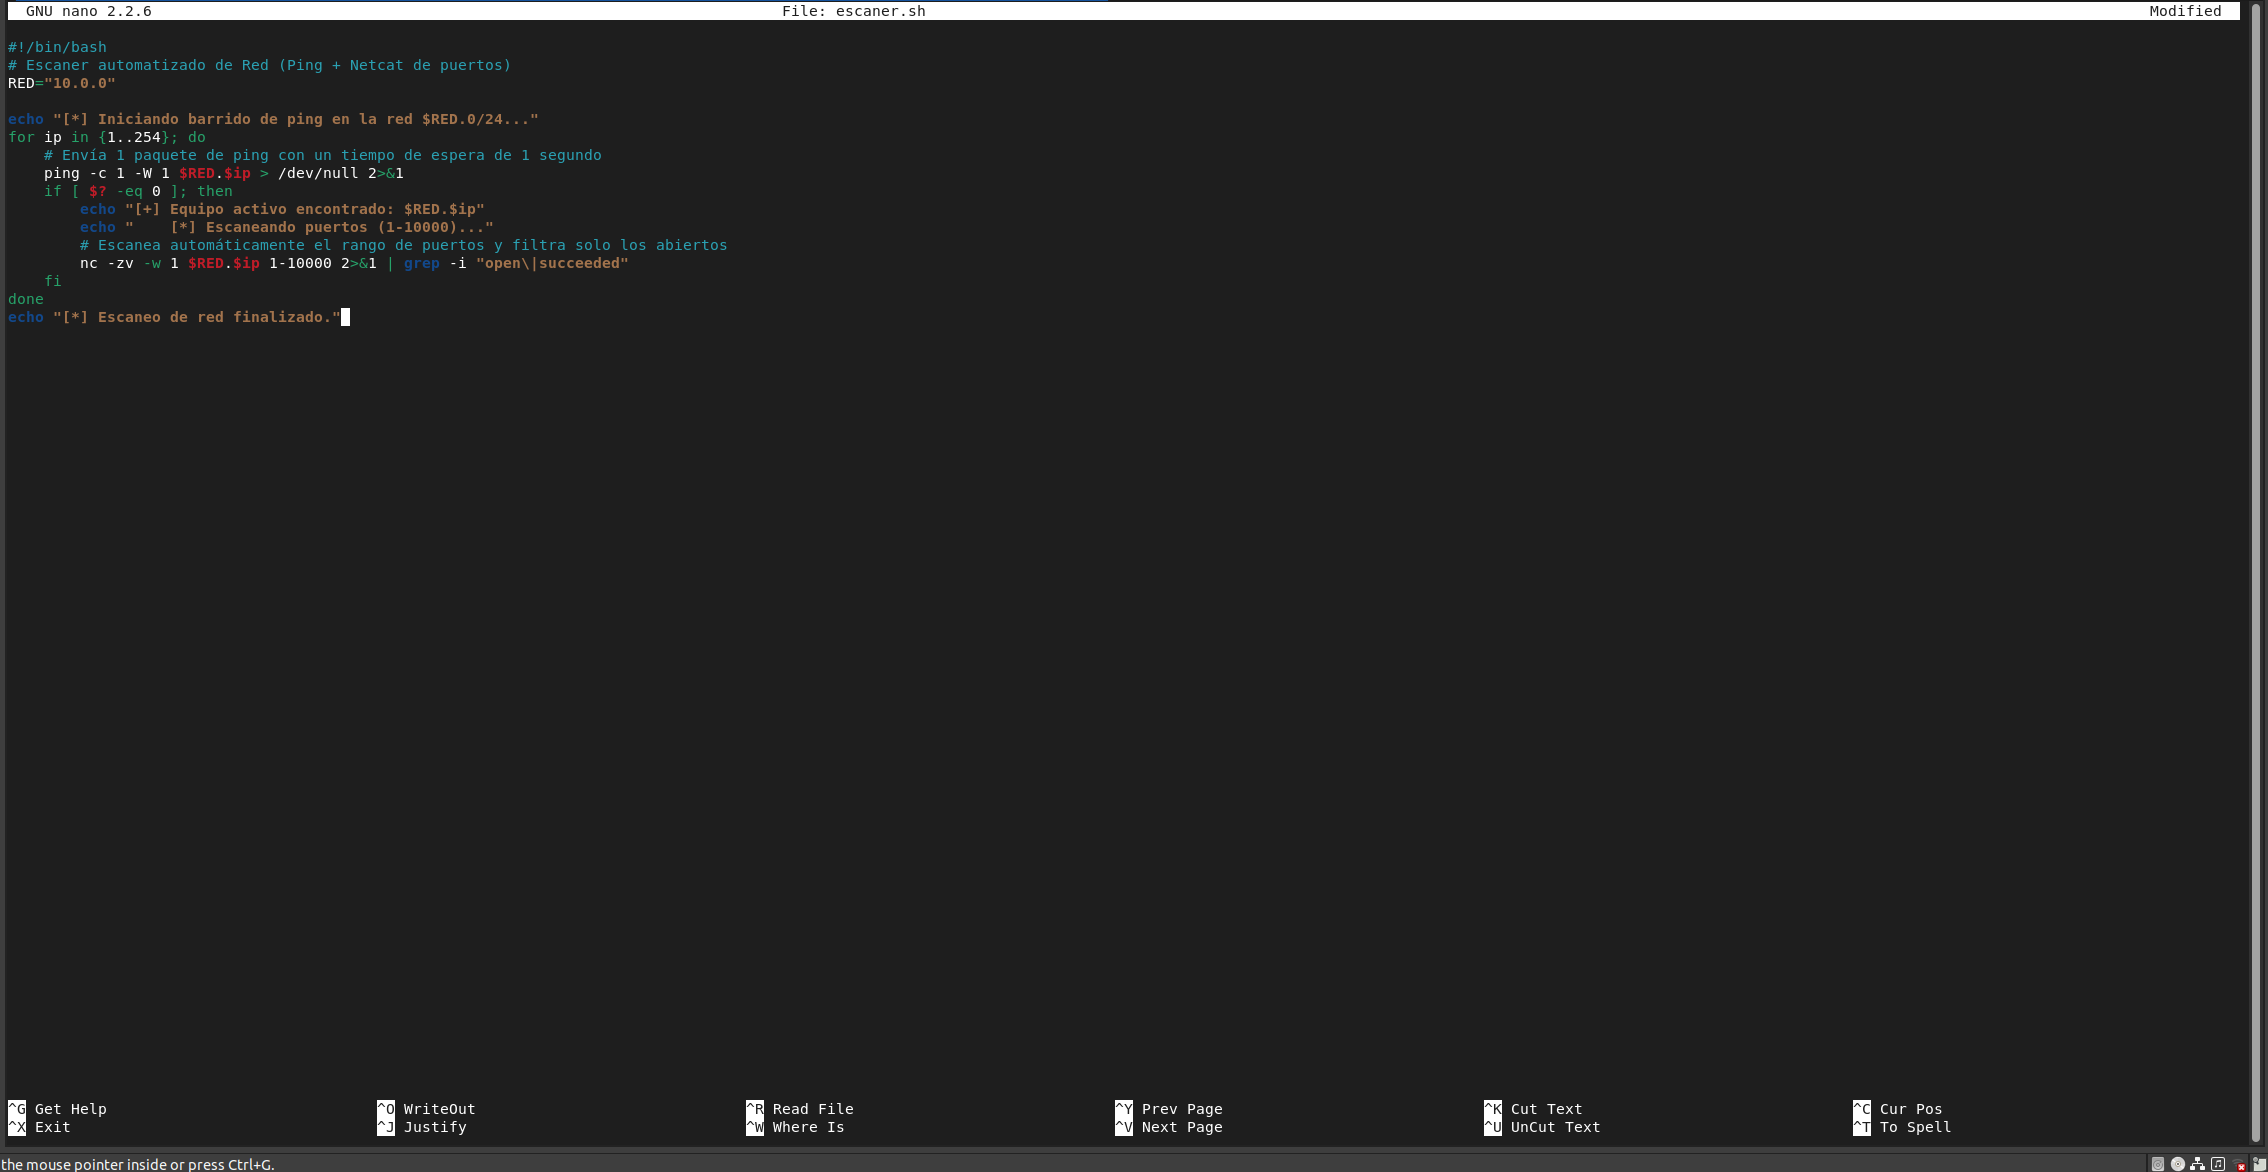
\includegraphics[width=\textwidth,trim=0bp 800bp 900bp 0bp,clip]{img/CapturasSeccionFinal/image3.png}
    \caption{Codigo del escaner de red en Bash.}
\end{figure}

Para entender lo que hace el programa, primero se define
\texttt{RED="10.0.0"}, siendo esta la parte de la direccion que no
cambia. Despues, el ciclo for recorre los valores del 1 al 254 y
forma las direcciones que se van a revisar, dejando fuera la
direccion de red y la de broadcast.

El comando \texttt{ping -c 1 -W 1} envia un solo paquete y espera
hasta un segundo por la respuesta. La redireccion \texttt{>
/dev/null 2>\&1} oculta tanto la salida normal como los errores de
ping. Despues, \texttt{\$?} contiene el codigo de salida del
ultimo comando y \texttt{-eq 0} comprueba si termino
correctamente.

Si el equipo responde, se ejecuta nc para revisar sus puertos TCP
del 1 al 10000. Donde \texttt{-z} comprueba los puertos sin
intercambiar datos de aplicacion, \texttt{-v} muestra informacion
del intento y \texttt{-w 1} establece un tiempo de espera de un
segundo. La parte \texttt{2>\&1} permite pasar tambien los
mensajes de error a la tuberia y grep conserva las lineas que
contienen open o succeeded.

No obstante, este escaner solo revisa puertos de los equipos que
respondieron al ping. Ademas de que, el rango termina en 10000 y
se utiliza TCP, por lo que los resultados corresponden a esas
condiciones de la busqueda.

Despues de guardar el archivo, se copio al servidor por medio de
scp. El comando completo es el siguiente:

\begin{lstlisting}[style=consolaSeguridad]
scp -P 13337 escaner.sh webadmin@192.168.177.129:/home/webadmin/
\end{lstlisting}

\begin{figure}[H]
    \centering
    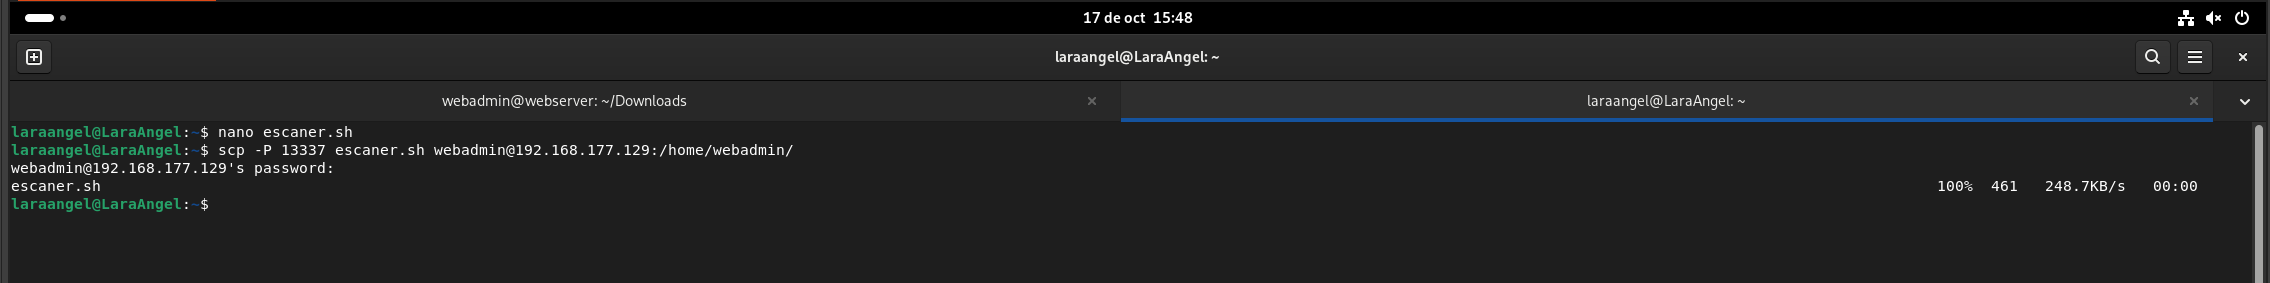
\includegraphics[width=\textwidth]{img/CapturasSeccionFinal/image1.png}
    \caption{Transferencia de escaner.sh desde EvilBox a webserver.}
\end{figure}

Donde \texttt{-P} indica el puerto SSH del servidor, escaner.sh es
el archivo local que se copia y \texttt{/home/webadmin/} es el
directorio de destino. Para autorizar la copia se utilizo la
contraseña de webadmin.

Una vez dentro de webserver, se revisaron los archivos con ls y se
dieron permisos de ejecucion al escaner:

\begin{lstlisting}[style=consolaSeguridad]
ls
chmod +x /home/webadmin/escaner.sh
\end{lstlisting}

\begin{figure}[H]
    \centering
    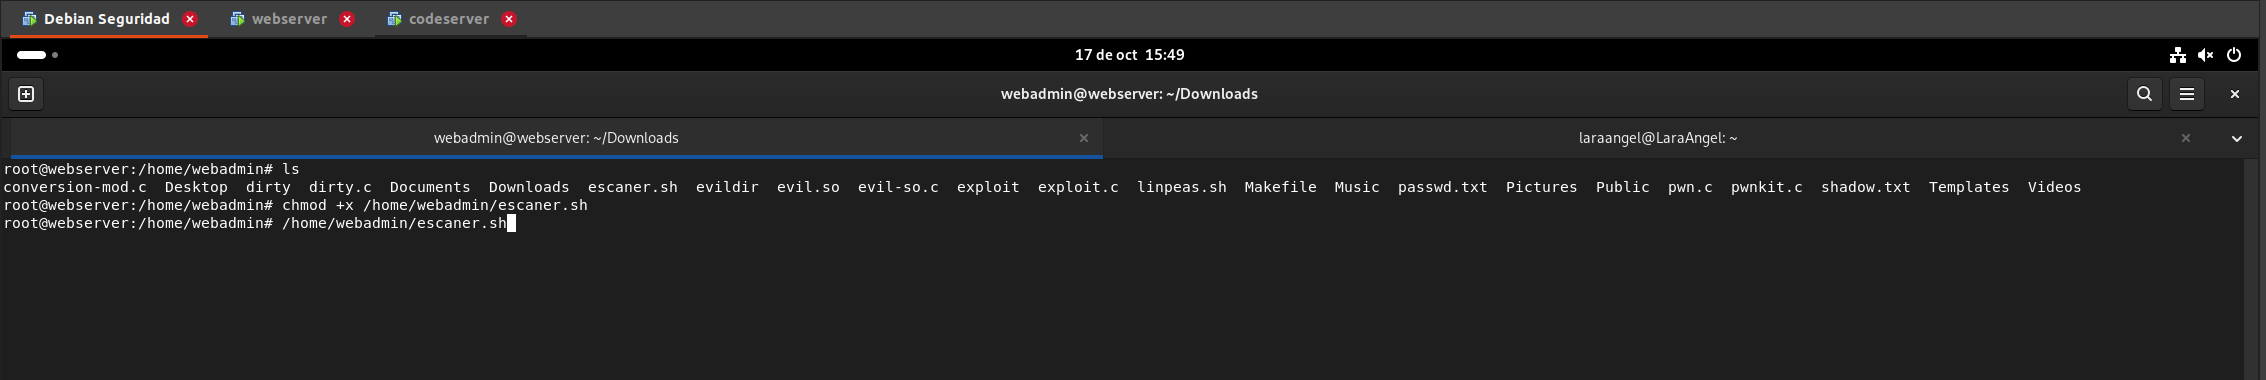
\includegraphics[width=\textwidth]{img/CapturasSeccionFinal/image2.png}
    \caption{Verificacion del archivo y asignacion del permiso de ejecucion.}
\end{figure}

Lo que hace \texttt{chmod +x} es agregar el permiso para ejecutar
el archivo. Despues de esto, desde el directorio de webadmin, se
pone el siguiente comando:

\begin{lstlisting}[style=consolaSeguridad]
./escaner.sh
\end{lstlisting}

\subsection{Equipos encontrados y revision de los servicios}

La salida del escaner nos arroja dos equipos activos en la red
interna, siendo \texttt{10.0.0.78} y \texttt{10.0.0.201}. Donde el
primero corresponde al mismo webserver por su interfaz eth1,
mientras que el segundo es el otro equipo encontrado.

\begin{lstlisting}[style=output]
Equipo activo encontrado: 10.0.0.78
111/tcp open
80/tcp open

Equipo activo encontrado: 10.0.0.201
5985/tcp open
3389/tcp open
445/tcp open
139/tcp open
135/tcp open
80/tcp open
\end{lstlisting}

Para el equipo distinto a webserver se encontraron seis puertos
TCP abiertos dentro del rango que reviso el escaner. Ahora bien,
para identificar mejor los servicios de los puertos 5985 y 3389,
se ejecutaron los siguientes comandos:

\begin{lstlisting}[style=consolaSeguridad]
sudo nmap -sV -p 5985 10.0.0.201
sudo nmap -sV -p 3389 10.0.0.201
\end{lstlisting}

Donde \texttt{-sV} intenta identificar el servicio y su version,
\texttt{-p} indica el puerto que se va a revisar y al final se
pone la direccion del equipo. Para el puerto 5985, nmap devuelve
lo siguiente:

\begin{lstlisting}[style=output]
PORT     STATE SERVICE VERSION
5985/tcp open  http    Microsoft HTTPAPI httpd 2.0 (SSDP/UPnP)
Service Info: OS: Windows
\end{lstlisting}

Por otro lado, para el puerto 3389 se obtiene el siguiente
resultado:

\begin{lstlisting}[style=output]
PORT     STATE SERVICE       VERSION
3389/tcp open  ms-wbt-server Microsoft Terminal Service
Service Info: OS: Windows
\end{lstlisting}

\begin{figure}[H]
    \centering
    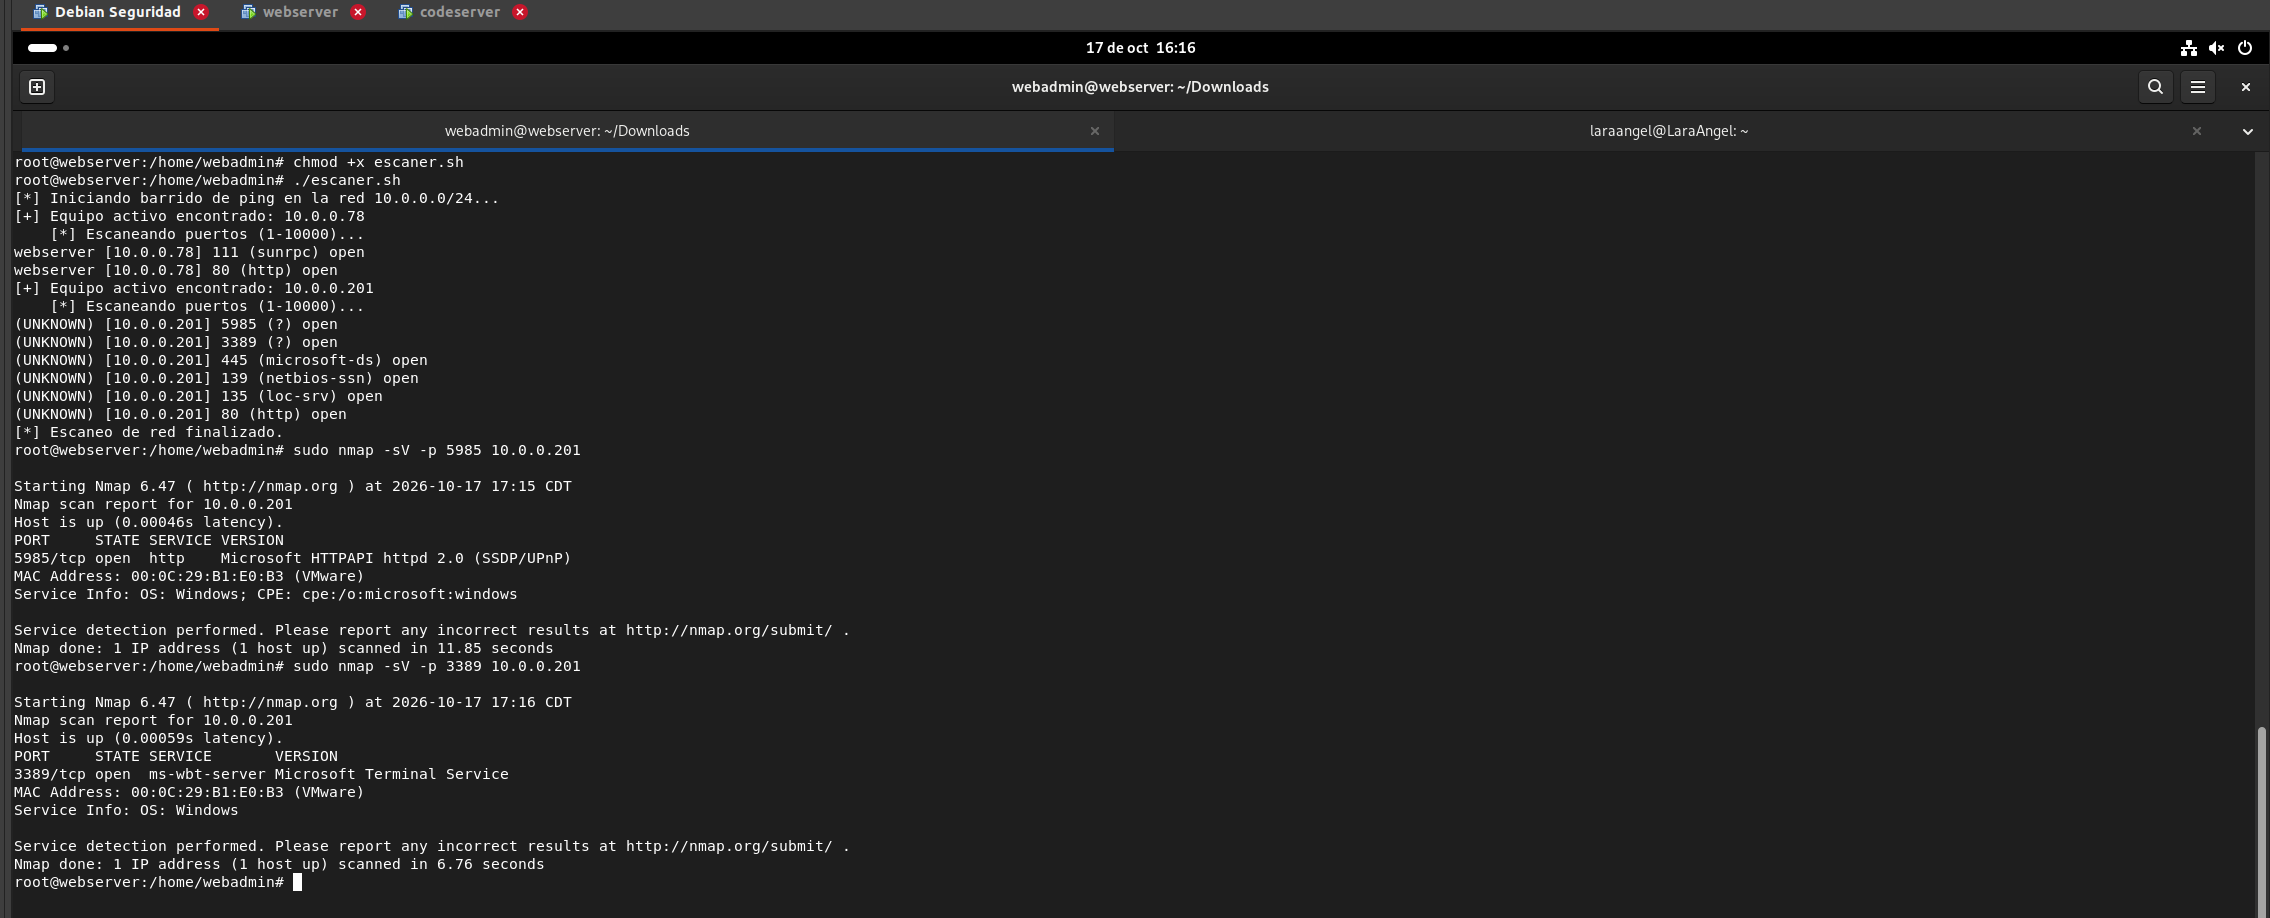
\includegraphics[width=\textwidth]{img/CapturasSeccionFinal/image4.png}
    \caption{Resultados del escaner e identificacion de los servicios en 10.0.0.201.}
\end{figure}

Con esto podemos ver servicios de Windows. El puerto 3389
corresponde a escritorio remoto y el 5985 devuelve Microsoft
HTTPAPI, coincidiendo con el puerto habitual de WinRM. Hasta
este punto se identificaron servicios, sin iniciar sesion en
el otro equipo.

\newpage\section{Actividades}

\subsection{Actividad 1: Version del kernel}

\textbf{¿Cual es la version del kernel del equipo webserver?}

Utilizamos el comando uname
que se ejecuto durante el desarrollo. El comando es el siguiente:

\Needspace{6\baselineskip}
\begin{lstlisting}[style=consolaSeguridad]
uname -v
\end{lstlisting}

\begin{lstlisting}[style=output]
#1 SMP Debian 3.16.56-1+deb8u1 (2018-05-08)
\end{lstlisting}

Donde en este caso, la version de compilacion obtenida es
\texttt{3.16.56-1+deb8u1}, con fecha del 8 de mayo del 2018. La
bandera utilizada fue \texttt{-v}, por lo que este valor
corresponde a la informacion de compilacion del kernel.

\begin{figure}[H]
    \centering
    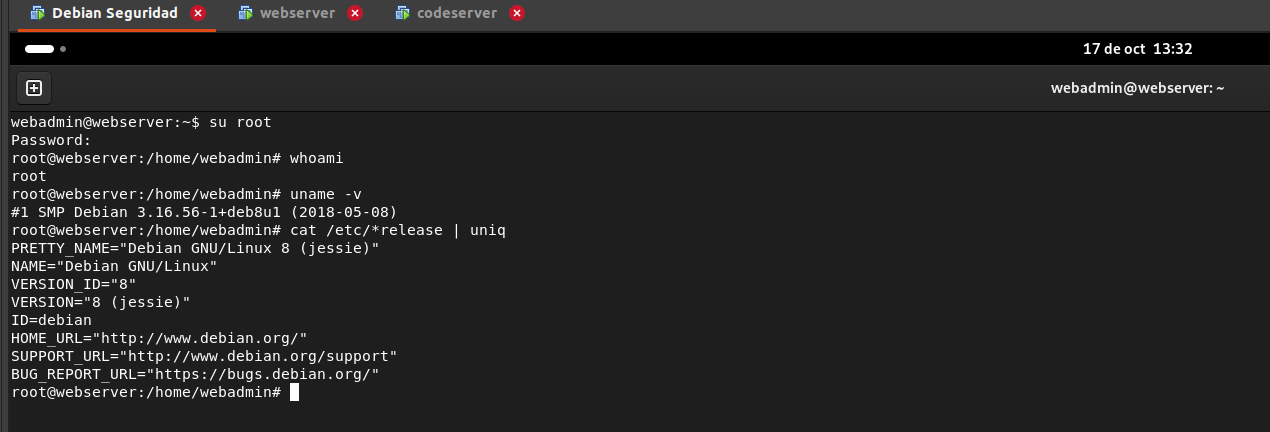
\includegraphics[width=\textwidth,trim=0bp 10bp 0bp 180bp,clip]{img/image5.png}
    \caption{Comprobacion de la version del kernel y de la distribucion.}
\end{figure}

\subsection{Actividad 2: Valor de PRETTY\_NAME}

\textbf{¿Cual es el valor de la variable PRETTY\_NAME?}

Para esto, revisamos el resultado del comando que muestra la
informacion de la distribucion:

\begin{lstlisting}[style=consolaSeguridad]
cat /etc/*release | uniq
\end{lstlisting}

\begin{lstlisting}[style=output]
PRETTY_NAME="Debian GNU/Linux 8 (jessie)"
\end{lstlisting}

Por lo que, el valor de PRETTY\_NAME es \texttt{Debian GNU/Linux 8
(jessie)}. Este campo contiene el nombre completo de la
distribucion instalada en webserver.

\Needspace{12\baselineskip}
\subsection{Actividad 3: Comando del servicio SSH}

\textbf{¿Cual es el comando que ejecuta el servicio SSH en el
equipo webserver?}

Para encontrarlo, revisamos la columna COMMAND del resultado de
ps, utilizando el siguiente comando:

\Needspace{6\baselineskip}
\begin{lstlisting}[style=consolaSeguridad]
ps aux awf
\end{lstlisting}

\begin{lstlisting}[style=output]
/usr/sbin/sshd -D
\end{lstlisting}

Donde \texttt{/usr/sbin/sshd} es el programa del servidor SSH y la
opcion \texttt{-D} hace que se mantenga en primer plano. El
proceso principal se ejecuta como root y tiene el PID 486.

\begin{figure}[H]
    \centering
    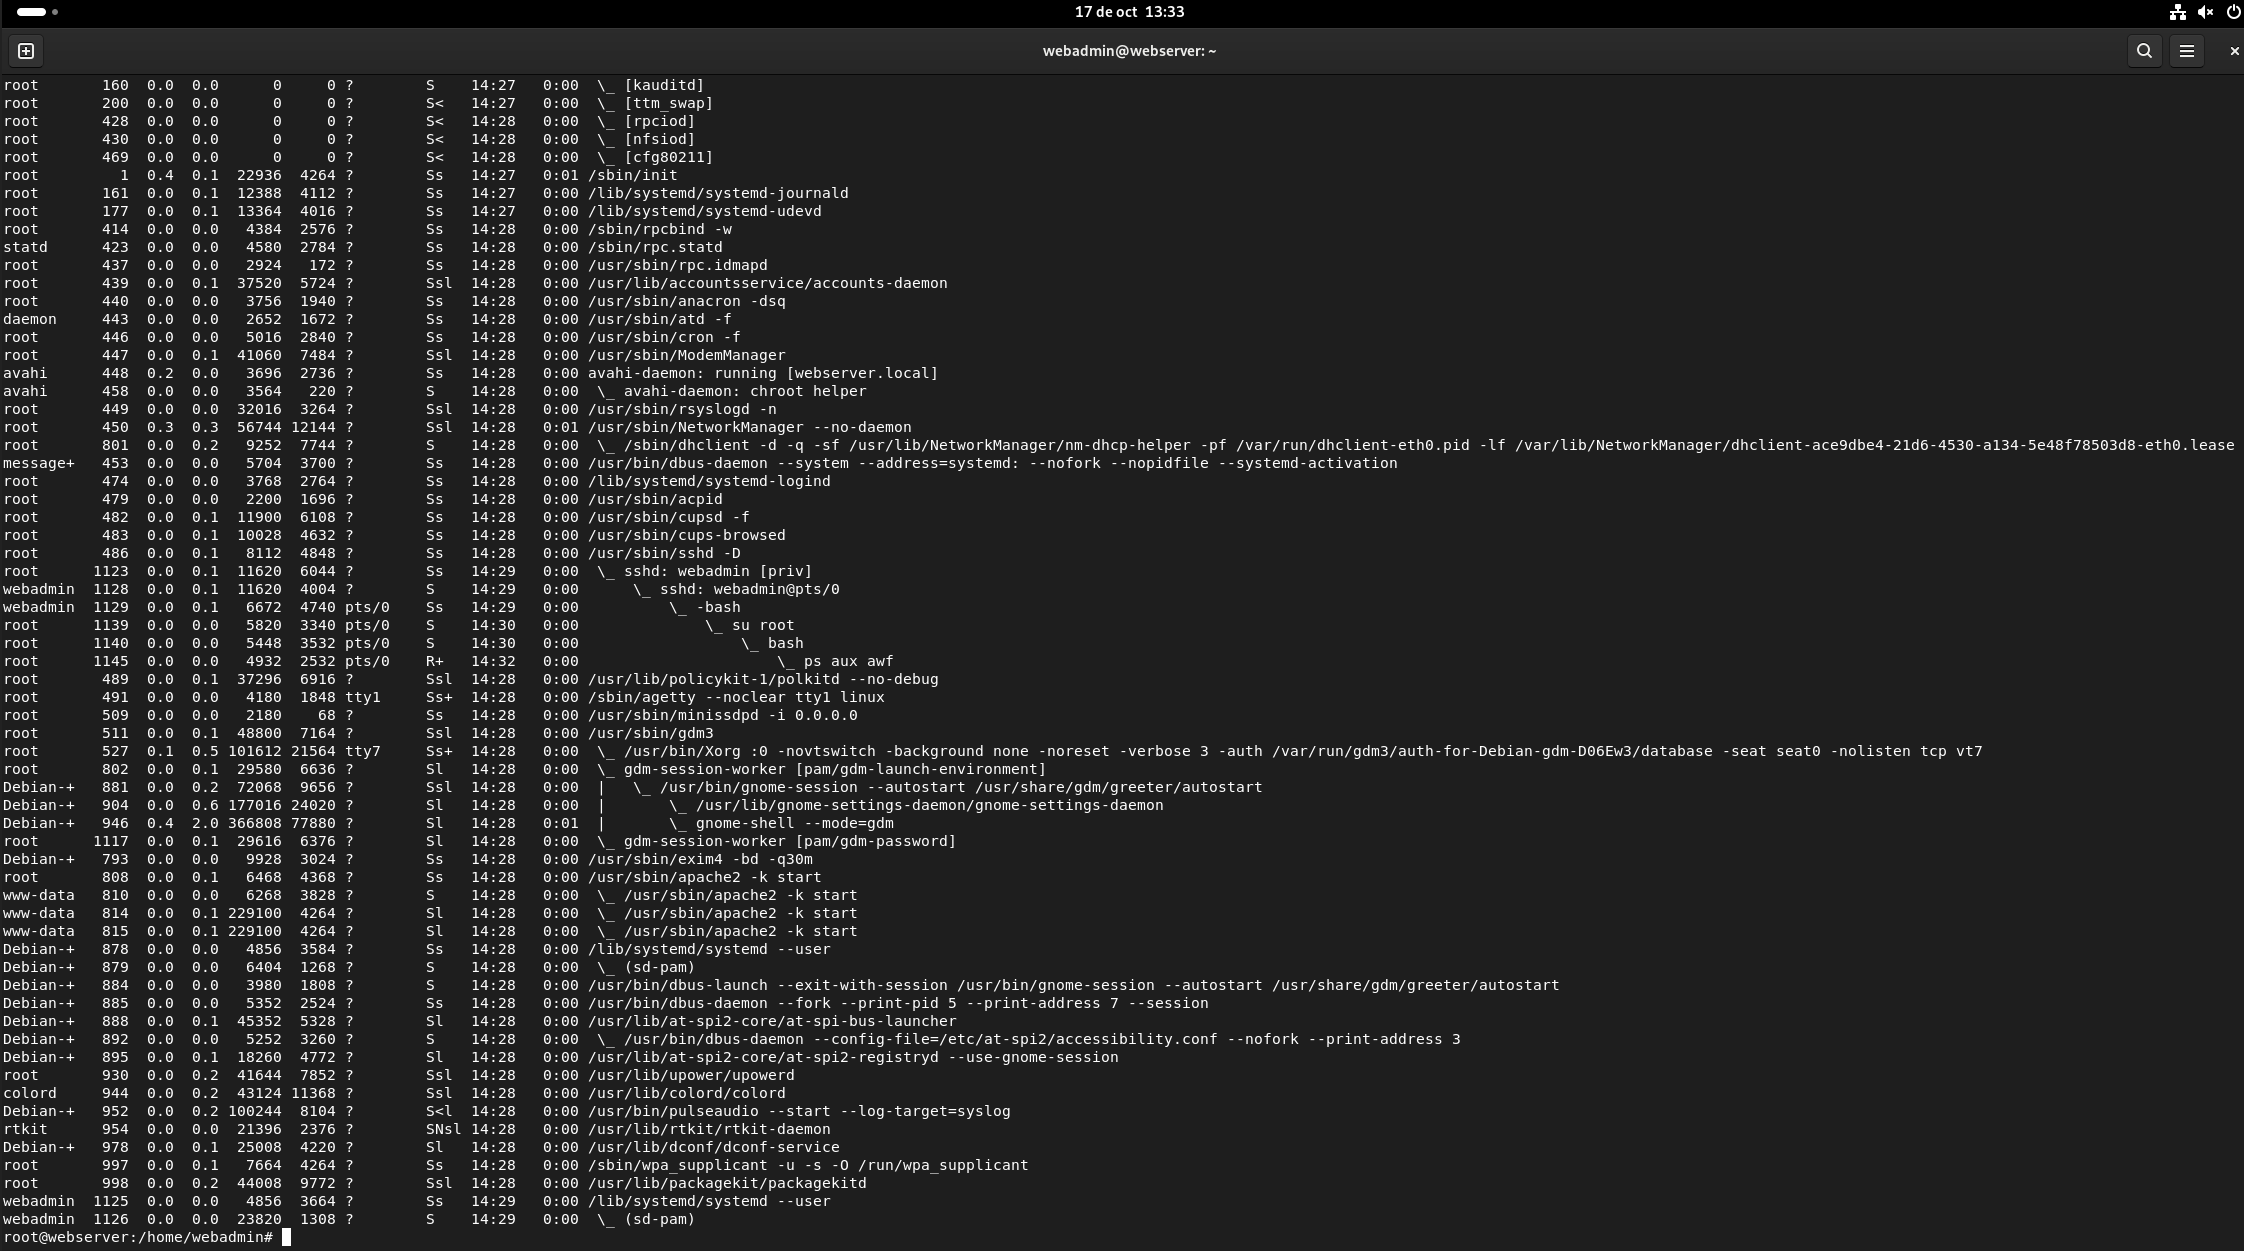
\includegraphics[width=\textwidth,trim=0bp 580bp 1360bp 540bp,clip]{img/image7.png}
    \caption{Proceso principal de SSH y procesos de la sesion de webadmin.}
\end{figure}

\subsection{Actividad 4: Comando del servicio Apache}

\textbf{¿Cual es el comando que ejecuta el servicio Apache en el
equipo webserver?}

De igual forma, en el listado que nos dio ps se identifica el
proceso de Apache. El comando que aparece es el siguiente:

\begin{lstlisting}[style=output]
/usr/sbin/apache2 -k start
\end{lstlisting}

Donde \texttt{/usr/sbin/apache2} es el programa del servidor web y
\texttt{-k start} indica el inicio del servicio. El proceso
principal tiene el PID 808 y se ejecuta como root, mientras que
los procesos hijos se ejecutan con el usuario www-data.

\begin{figure}[H]
    \centering
    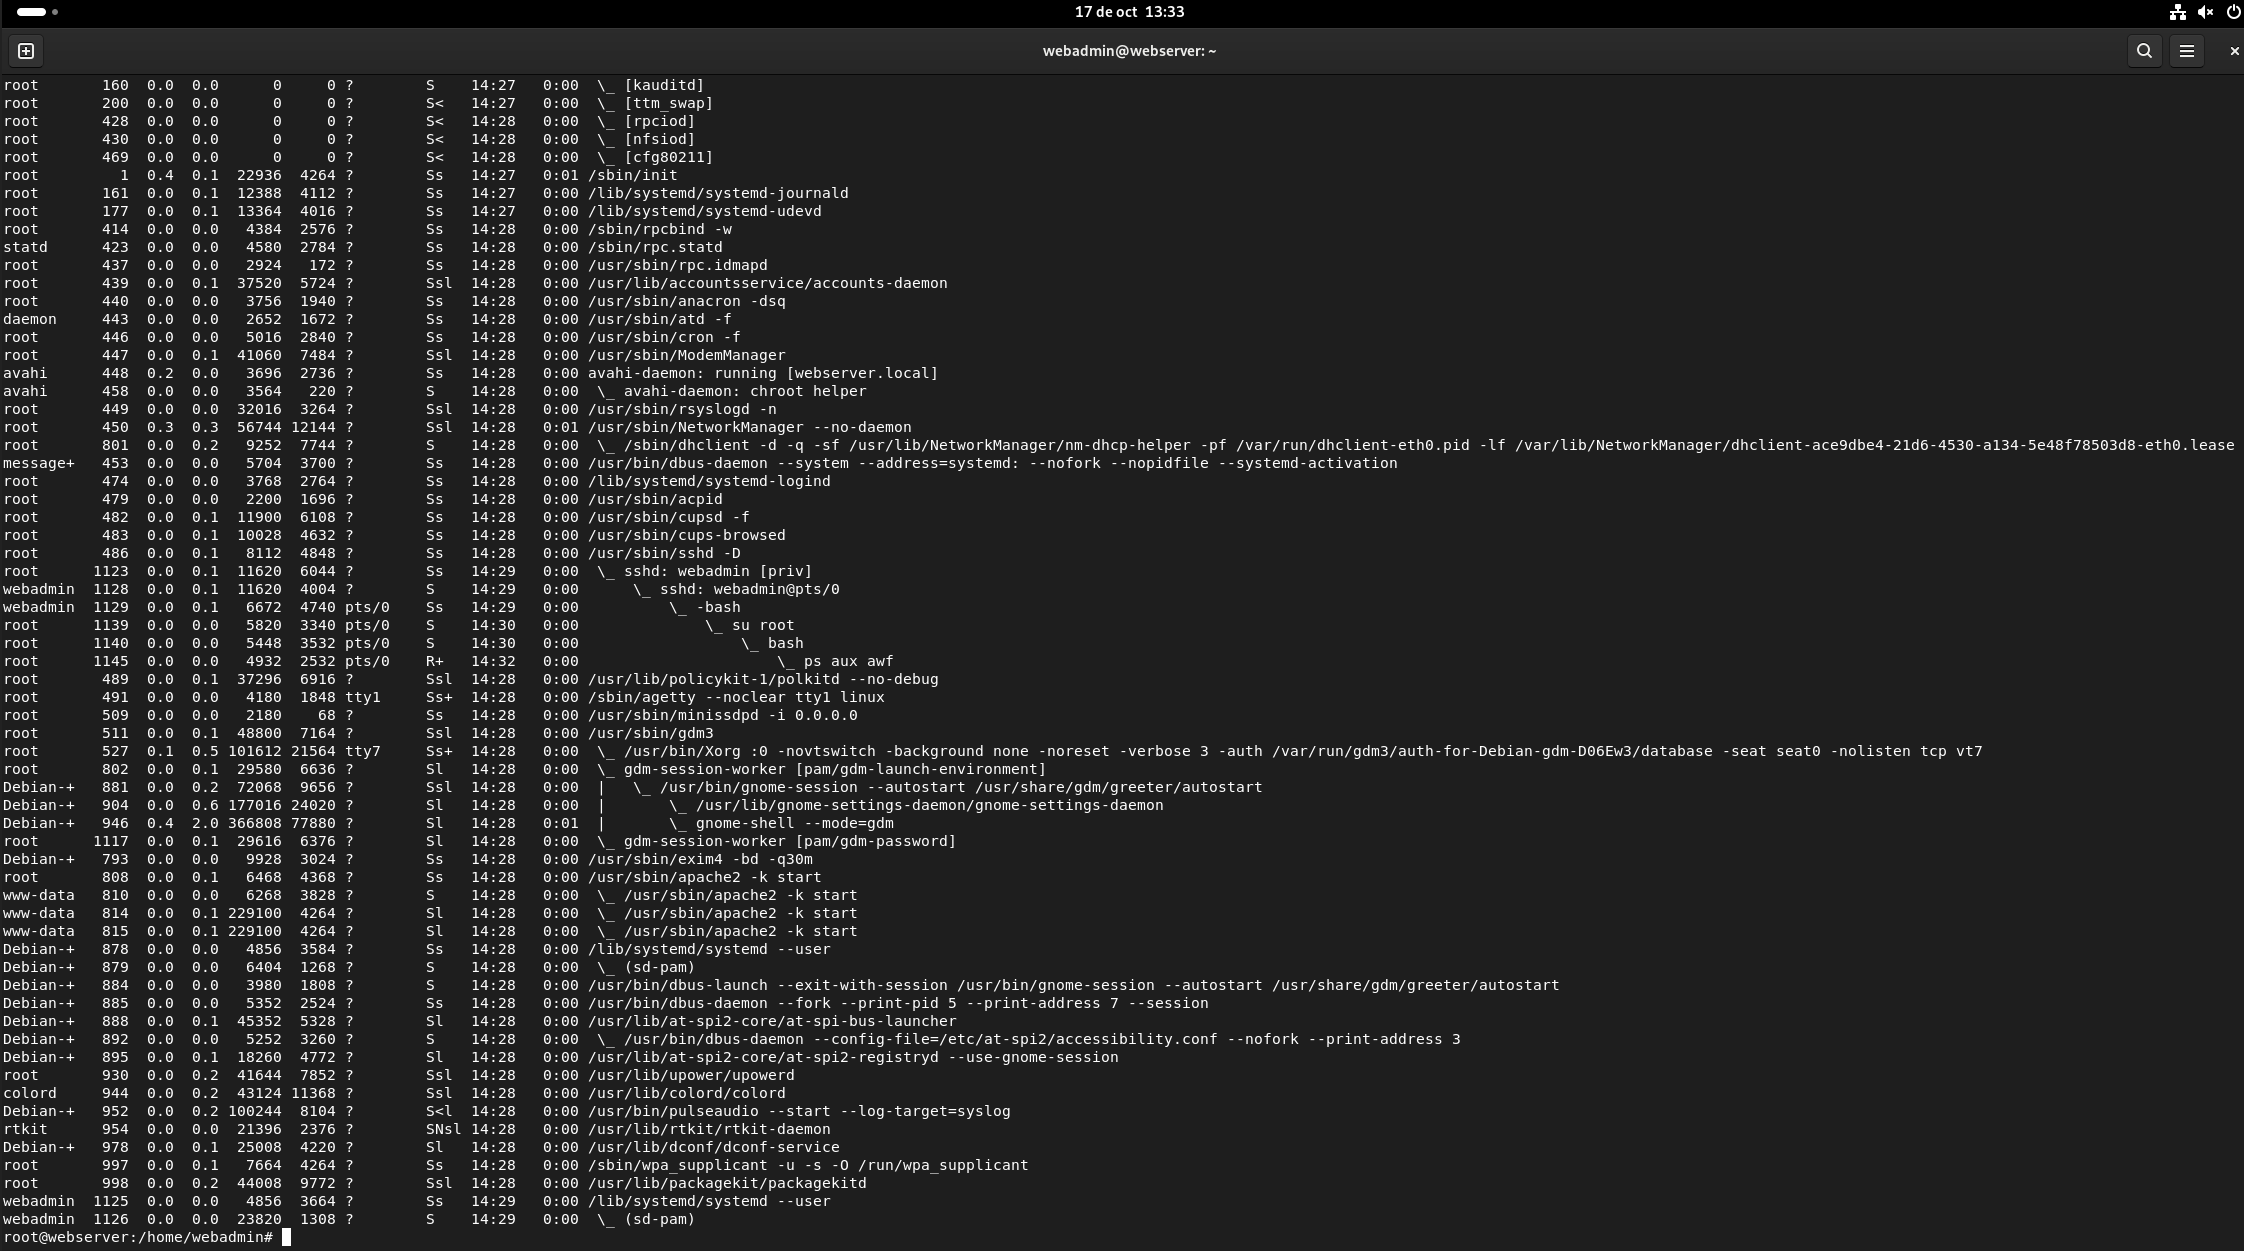
\includegraphics[width=\textwidth,trim=0bp 305bp 1300bp 865bp,clip]{img/image7.png}
    \caption{Proceso principal de Apache y procesos hijos de www-data.}
\end{figure}

\subsection{Actividad 5: Interfaces de red configuradas}

\textbf{¿Cuantas interfaces de red estan configuradas en el equipo
webserver?}

Para esto, utilizamos el resultado del siguiente comando:

\begin{lstlisting}[style=consolaSeguridad]
ifconfig -a
\end{lstlisting}

El equipo tiene \textbf{tres interfaces}, siendo \texttt{eth0},
\texttt{eth1} y \texttt{lo}. Donde las dos primeras son interfaces
Ethernet y la tercera es la interfaz de loopback. Por lo que, si
se cuentan solamente las interfaces Ethernet son dos, pero el
total que devuelve ifconfig -a es tres.

\begin{figure}[H]
    \centering
    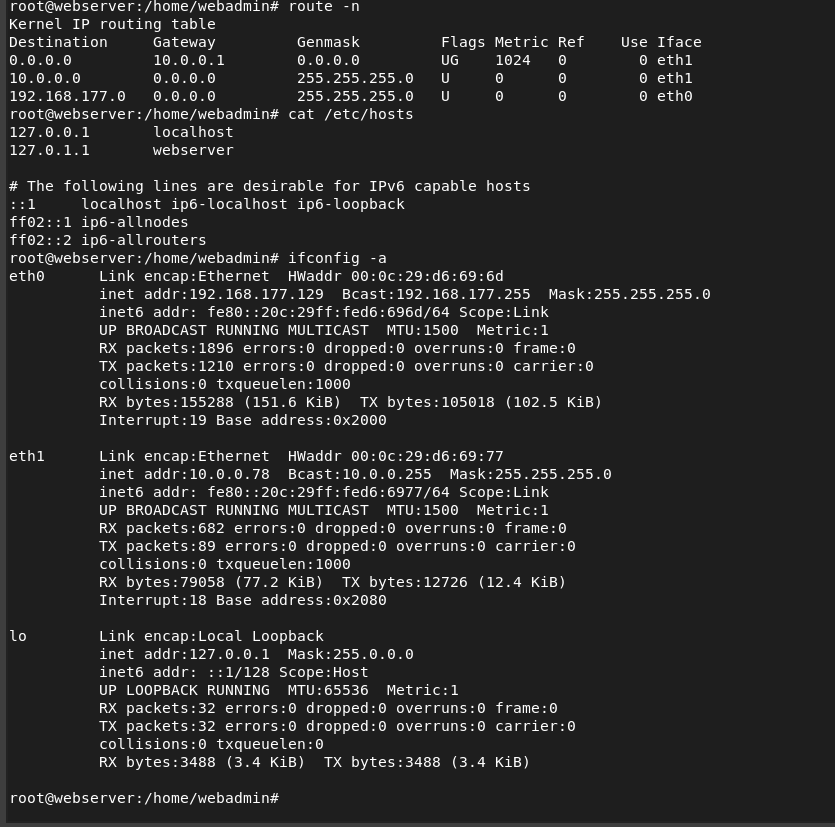
\includegraphics[width=0.84\textwidth,trim=0bp 0bp 0bp 247bp,clip]{img/image8.png}
    \caption{Interfaces eth0, eth1 y lo configuradas en webserver.}
\end{figure}

\subsection{Actividad 6: Direccion de la interfaz eth1}

\textbf{¿Cual es la direccion IP configurada en la interfaz eth1?}

Dentro de la informacion de ifconfig -a se revisa el apartado de
eth1. Donde en este caso, los datos son los siguientes:

\begin{lstlisting}[style=output]
eth1
inet addr:10.0.0.78
Bcast:10.0.0.255
Mask:255.255.255.0
\end{lstlisting}

Por lo que la direccion IP de eth1 es \textbf{10.0.0.78}, con
mascara \texttt{255.255.255.0}. Esto nos permite identificar que
la red interna a revisar es \texttt{10.0.0.0/24}.

\subsection{Actividad 7: Ruta del archivo con contraseñas en claro}

\textbf{¿Cual es la ruta absoluta del archivo que contiene
contraseñas en claro?}

Para encontrar el archivo, primero se amplio la busqueda de
nombres con el comando siguiente:

\begin{lstlisting}[style=consolaSeguridad]
find / -type f -iname "*pass*.txt" 2>/dev/null
\end{lstlisting}

Despues se reviso el contenido del archivo passwords.txt con cat.
La ruta absoluta es la siguiente:

\begin{lstlisting}[style=output]
/home/webadmin/Downloads/home/developer2024/ProjectX/ProjectX_CodeBackup/config/passwords.txt
\end{lstlisting}

El archivo contiene diez pares de usuario y contraseña, entre
ellos \texttt{usuario1: 12345}, \texttt{admin: qwerty} y
\texttt{developer2024: R0b0tRulz!}. Con esto se comprobo que son
contraseñas en claro y no hashes como los que se obtuvieron de
shadow en la practica anterior.

\begin{figure}[H]
    \centering
    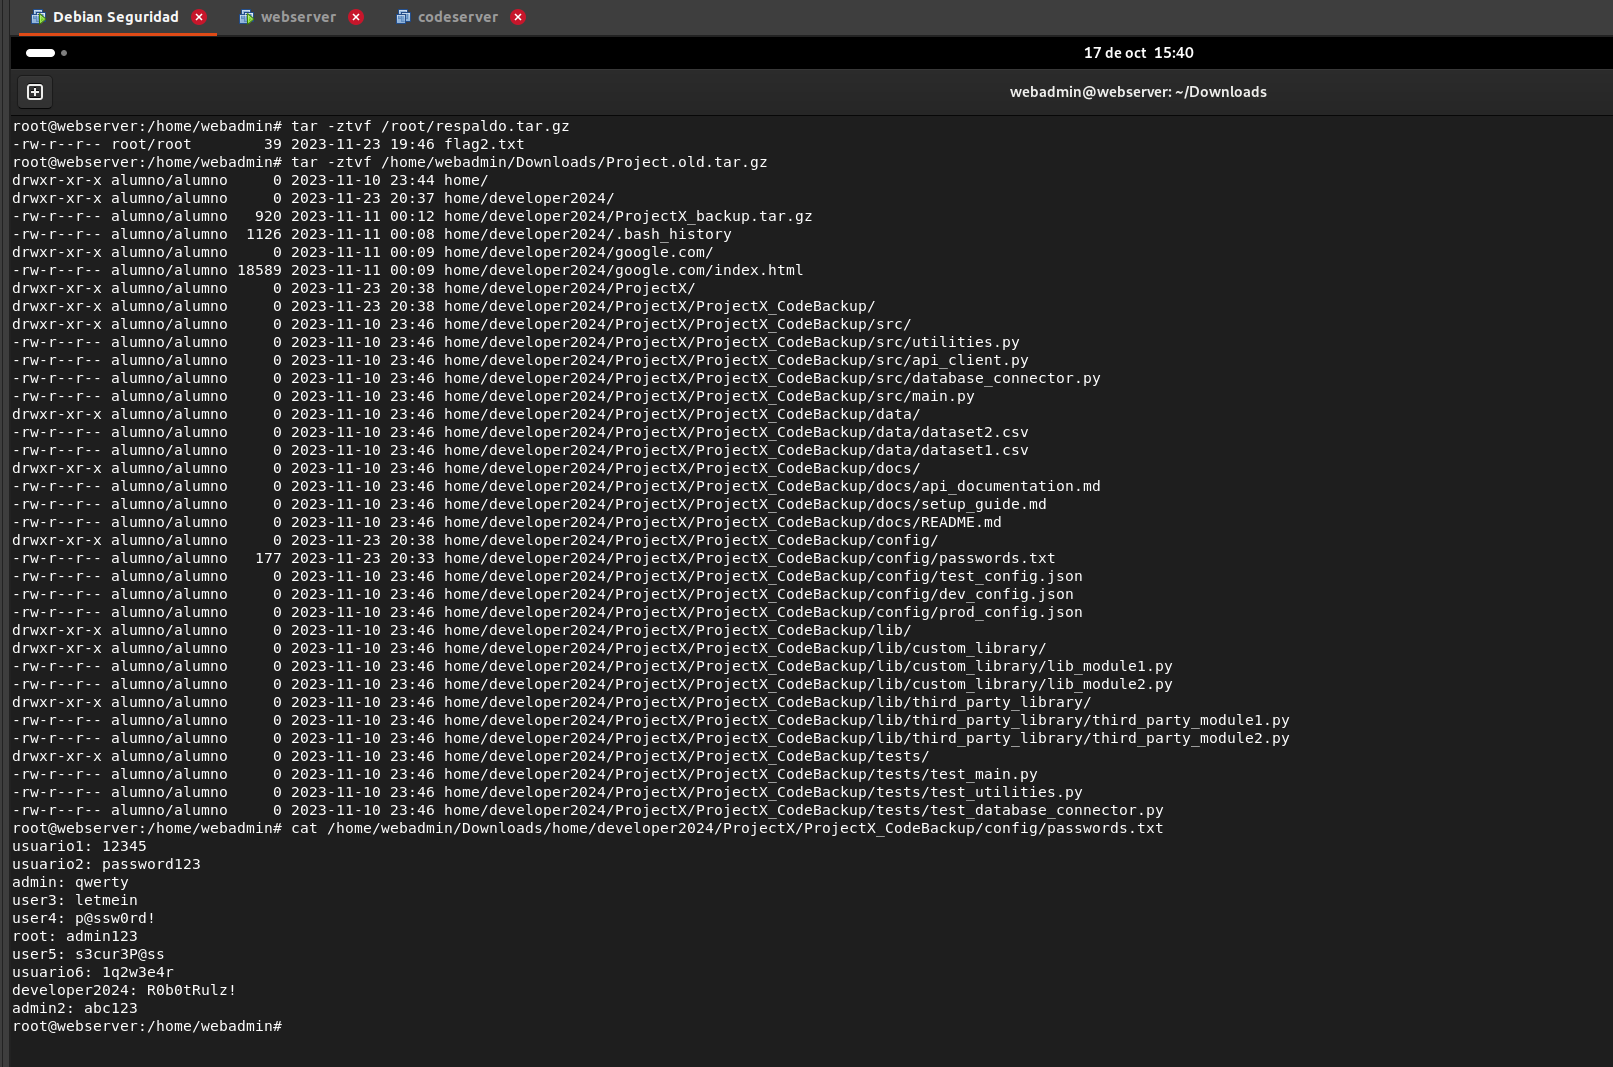
\includegraphics[width=\textwidth,trim=0bp 0bp 0bp 815bp,clip]{img/parte9Desarrollo/image12.png}
    \caption{Ruta y contenido del archivo passwords.txt.}
\end{figure}

\subsection{Actividad 8: Otro equipo en la red interna}

\textbf{¿Cual es la direccion IP del equipo distinto a webserver
que esta conectado a la misma red configurada en la interfaz
eth1?}

Se utilizo el escaner desde
webserver sobre la red 10.0.0.0/24. La ejecucion se realizo con el
siguiente comando:

\begin{lstlisting}[style=consolaSeguridad]
./escaner.sh
\end{lstlisting}

\begin{lstlisting}[style=output]
Equipo activo encontrado: 10.0.0.78
Equipo activo encontrado: 10.0.0.201
\end{lstlisting}

Donde \texttt{10.0.0.78} es la direccion de eth1 del mismo
webserver. Por lo tanto, la direccion del otro equipo encontrado
es \textbf{10.0.0.201}, correspondiente al equipo que se buscaba
en la red interna.

\begin{figure}[H]
    \centering
    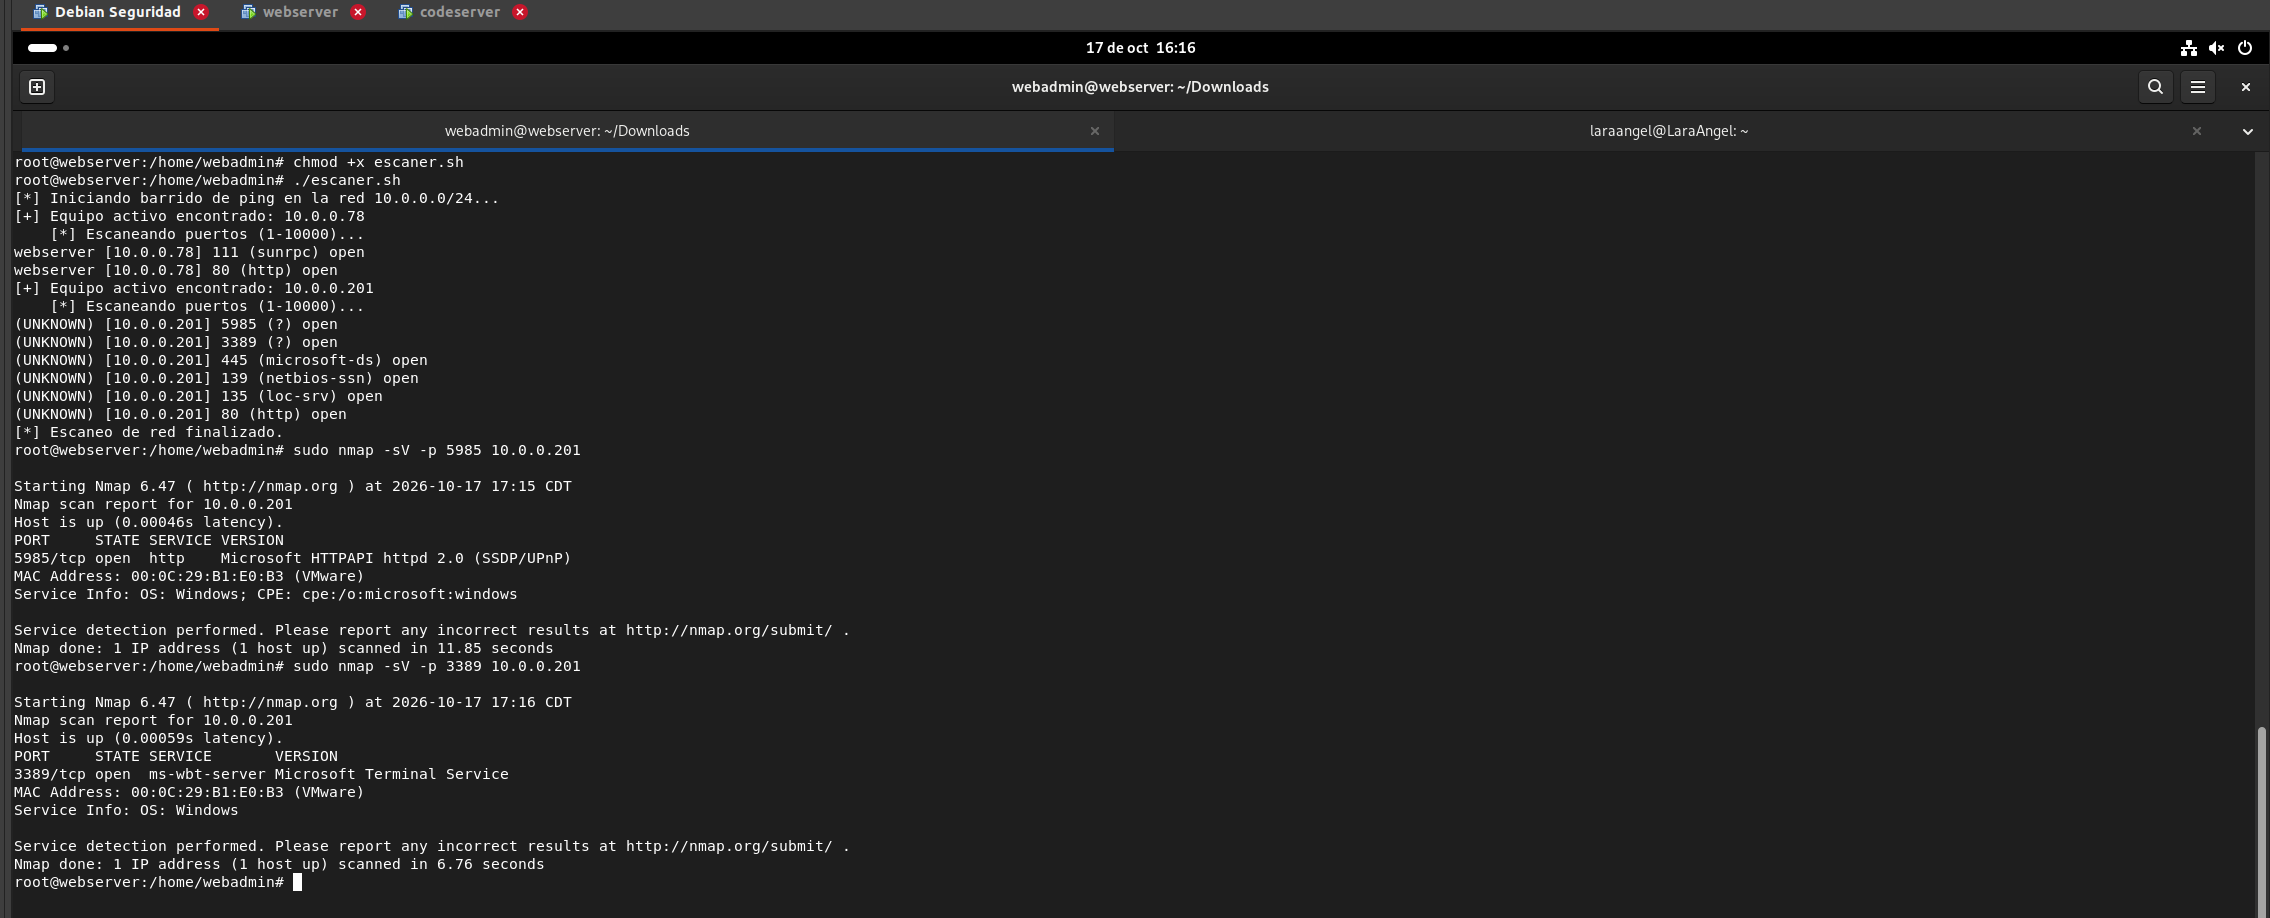
\includegraphics[width=\textwidth,trim=0bp 480bp 1100bp 150bp,clip]{img/CapturasSeccionFinal/image4.png}
    \caption{Equipo distinto a webserver y puertos encontrados en la red interna.}
\end{figure}

\subsection{Actividad 9: Puertos a la escucha del otro equipo}

\textbf{¿Cuantos puertos a la escucha estan configurados en el
equipo distinto a webserver que esta conectado a la misma red
configurada en la interfaz eth1?}

Para esto, tomamos los resultados de nc para 10.0.0.201. Donde en
este caso se encontraron \textbf{seis puertos TCP abiertos},
siendo los siguientes:

\begin{center}
\begin{tabular}{|c|l|}
\hline
\textbf{Puerto TCP} & \textbf{Servicio o asociacion habitual} \\ \hline
80 & HTTP \\ \hline
135 & RPC de Windows \\ \hline
139 & NetBIOS \\ \hline
445 & SMB \\ \hline
3389 & Escritorio remoto, confirmado con nmap \\ \hline
5985 & Puerto habitual de WinRM sobre HTTP \\ \hline
\end{tabular}
\end{center}

Este conteo corresponde al rango del 1 al 10000 que se reviso con
el escaner. Por lo que la respuesta obtenida es seis dentro de ese
rango; no se revisaron los puertos TCP superiores a 10000 ni
puertos UDP.

\subsection{Actividad 10: Puerto para establecer una sesion remota}

\textbf{¿Cual es el puerto que permite establecer una sesion
remota al equipo distinto a webserver que esta conectado a la
misma red configurada en la interfaz eth1?}

Para la administracion remota por WinRM, el puerto identificado es
\textbf{5985/TCP}. Para revisar el servicio que responde en ese
puerto se utilizo el comando siguiente:

\begin{lstlisting}[style=consolaSeguridad]
sudo nmap -sV -p 5985 10.0.0.201
\end{lstlisting}

\begin{lstlisting}[style=output]
5985/tcp open http Microsoft HTTPAPI httpd 2.0 (SSDP/UPnP)
\end{lstlisting}

Donde el puerto coincide con el que utiliza WinRM por HTTP. No
obstante, tambien se encontro abierto el \textbf{3389/TCP}, que
permite escritorio remoto y se identifico con el siguiente
comando:

\begin{lstlisting}[style=consolaSeguridad]
sudo nmap -sV -p 3389 10.0.0.201
\end{lstlisting}

\begin{lstlisting}[style=output]
3389/tcp open ms-wbt-server Microsoft Terminal Service
\end{lstlisting}

Por lo que, para una sesion de administracion por WinRM se
considera el puerto 5985, mientras que para una sesion grafica de
escritorio remoto se tiene el puerto 3389. En esta parte se
identificaron los servicios, sin realizar todavia una conexion
autenticada al otro equipo.


\newpage
\nocite{*}
\printbibliography[heading=bibintoc,title={Referencias}]
\end{document}
